\documentclass[12pt]{article}

\usepackage{graphicx}
\usepackage[font=footnotesize]{subfig}
\usepackage{float}
\usepackage{xepersian}
\settextfont[Scale=1]{XB Niloofar}
\setlatintextfont[Scale=1]{Times New Roman}
\title{پروژه پایانی درس الگوریتم‌های معاملاتی}
\author{فرزان مسیبی، کورش تقی‌پور پاسدار}


\begin{document}
	\maketitle
	\newpage
	\tableofcontents
	\newpage
	\section{جمع‌آوری مجموعه دادگان}
	بر طبق مساله طرح شده، برای ساخت پورتفولیو، داده‌های تاریخی ۴ رمزارز \lr{BTC-USD}، \lr{ETH-USD}، \lr{BNB-USD} و \lr{XRP-USD} در بازه زمانی \date{01 آگوست 2023} تا \date{01 دسامبر 2024} در بازه‌های زمانی روزانه دریافت شدند و همچنین داده‌های \lr{Null} نیز حذف شدند. این داده‌ها به دو بخش آموزش و تست تقسیم شدند.
	\begin{itemize}
		\item[بخش آمورش] از تاریخ \date{01 آگوست 2023} تا \date{01 آگوست 2024}
		\item[بخش تست] از تاریخ \date{01 آگوست 2024} تا \date{01 دسامبر 2024}
	\end{itemize}
	\begin{figure}[h!]
		\centering
		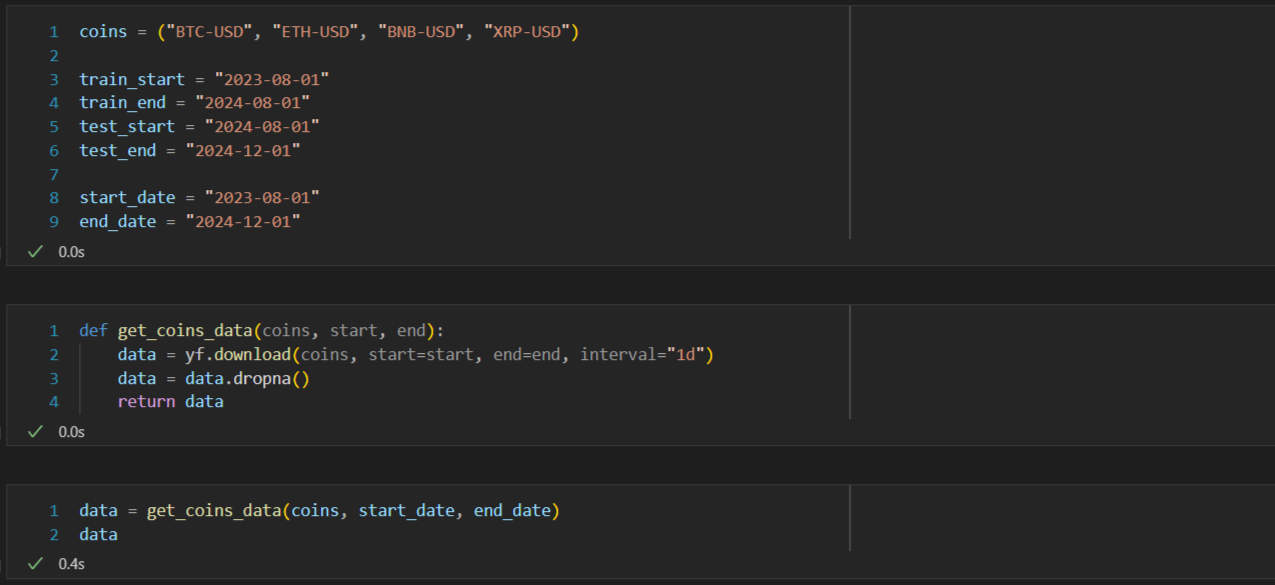
\includegraphics[width=0.9\linewidth]{pic_1}
		\caption{دریافت داده‌ها}
	\end{figure}
	داده‌های دریافتی چهار رمزارز بصورت روزانه، و شامل داده‌های \lr{Open}، \lr{Close}، \lr{High} و \lr{Low} هستند.
	\begin{figure}[H]
		\centering
		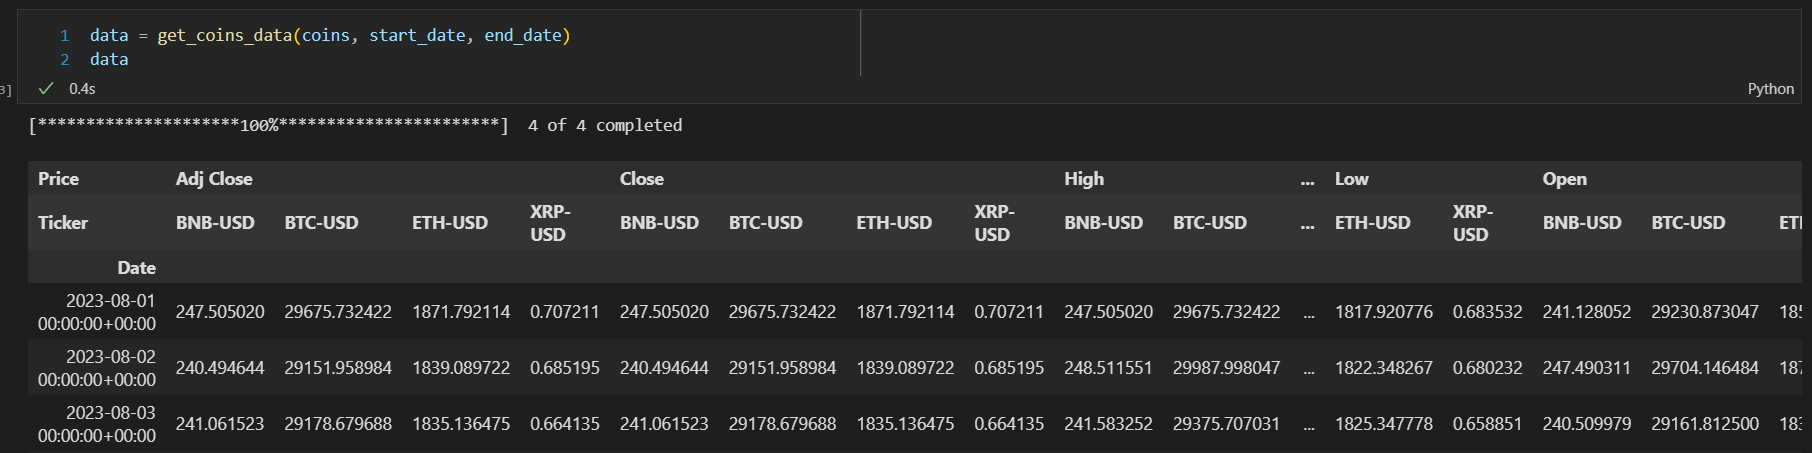
\includegraphics[width=0.9\linewidth]{pic_2}
	\end{figure}
	همچنین داده‌ها را با استفاده از کتابخانه \lr{Matplotlib} رسم می‌کنیم.
\begin{figure}[H]
	\centering
	\subfloat[
	کد مربوط به ترسیم داده‌ها
	]{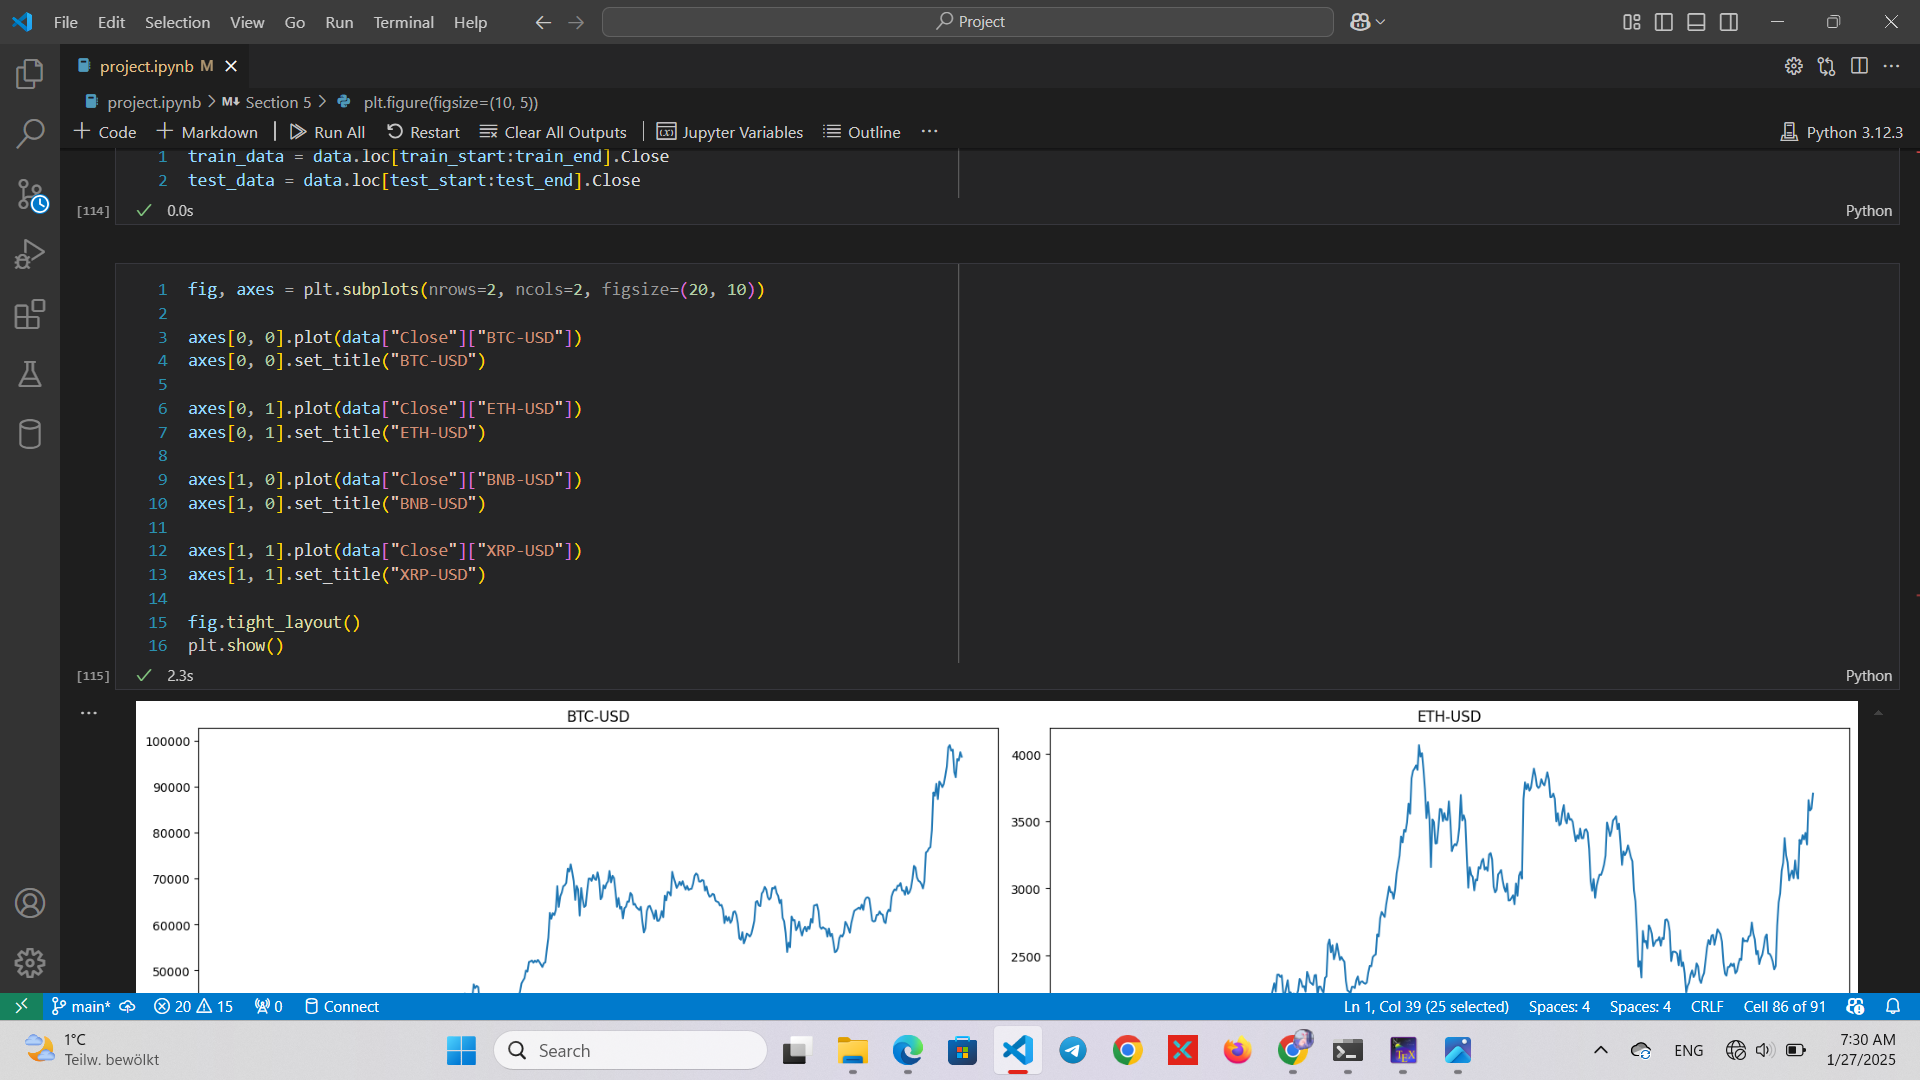
\includegraphics[width=0.4\linewidth]{pic_4}}
	\quad \quad
	\subfloat[
	نمودار رمزارزها
	]{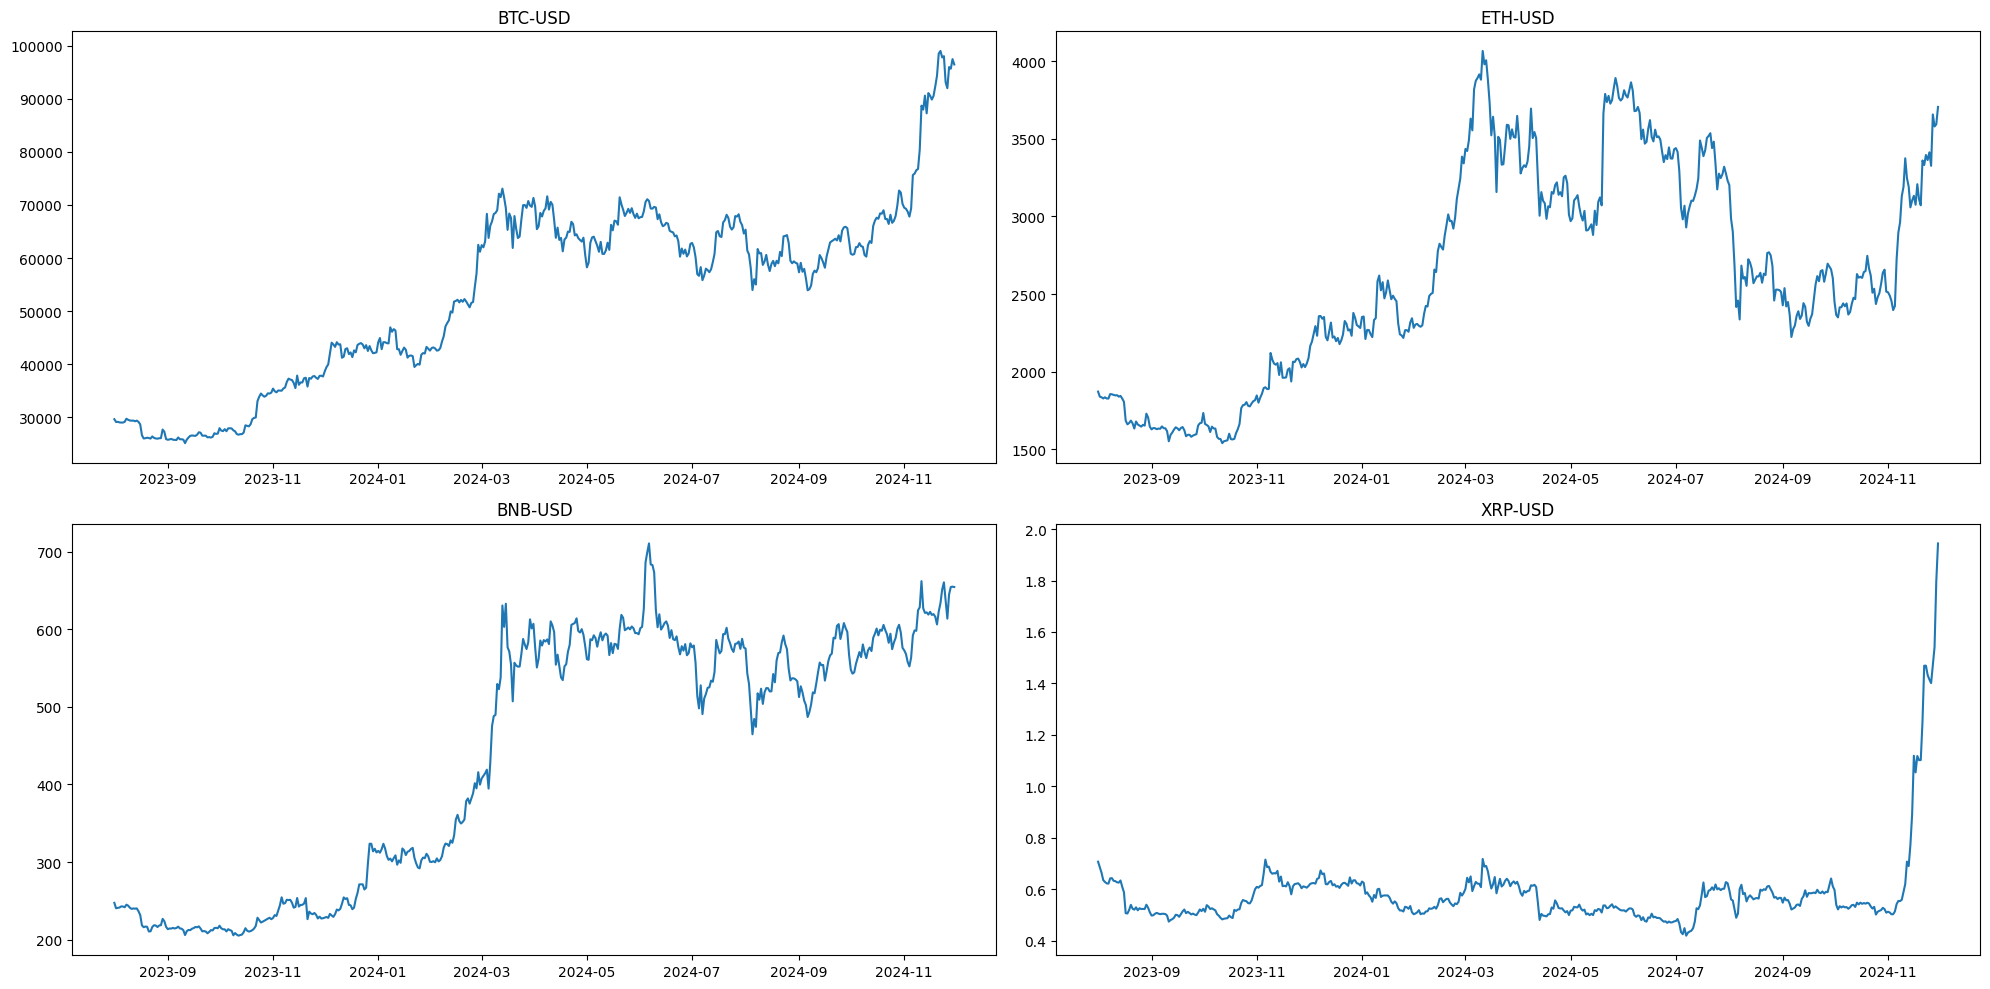
\includegraphics[width=0.4\linewidth]{pic_5}}
\end{figure}
\section{تخمین نوسان (\lr{Volatility Prediction})}
برای تخمین نوسان، دو راه معرفی شده است که مراحل طی شده برای هر دو توضیح داده می‌شوند.
\subsection{پیش‌بینی نوسان با استفاده از مدل‌های آماری}
در این روش، با استفاده از مدل‌های آماری \lr{GARCH}، \lr{EGARCH} و \lr{FIGARCH} نوسان را برای دو پنجره ذکر شده روی داده‌های آموزش پیش‌بینی می‌کنیم.
\begin{figure}[H]
	\centering
	\subfloat[
	پیش‌بینی نوسان برای دو پنجره ذکر شده.
	]{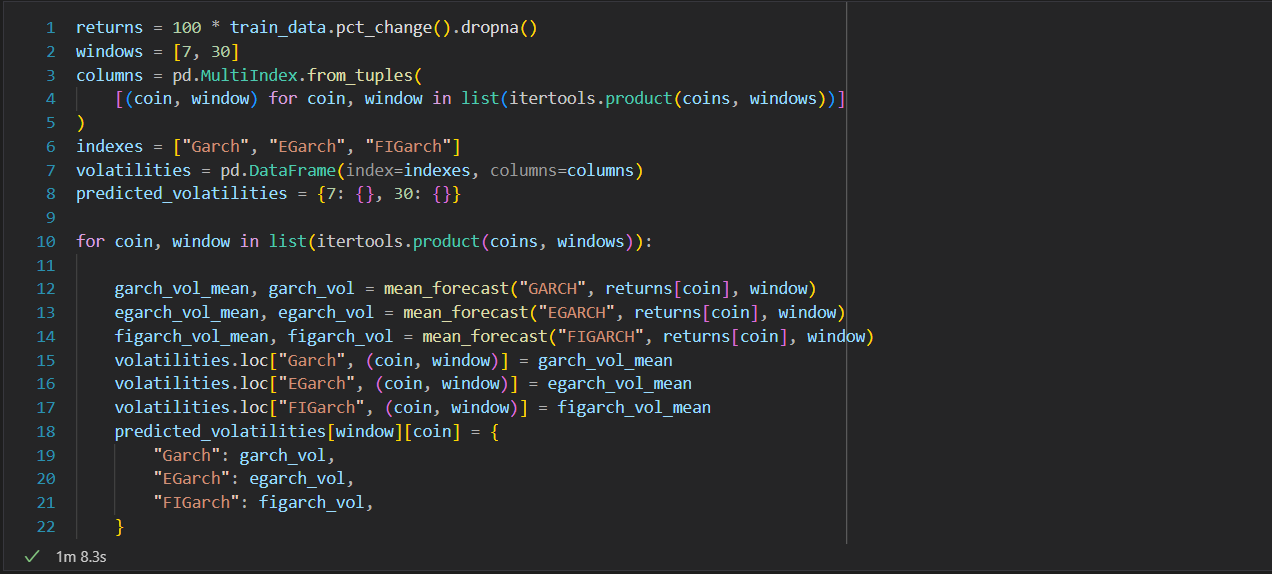
\includegraphics[width=0.4\linewidth]{pic_6}}
	\quad \quad
	\subfloat[
	تابعی برای محاسبه میانگین نوسان در هر پنجره
	]{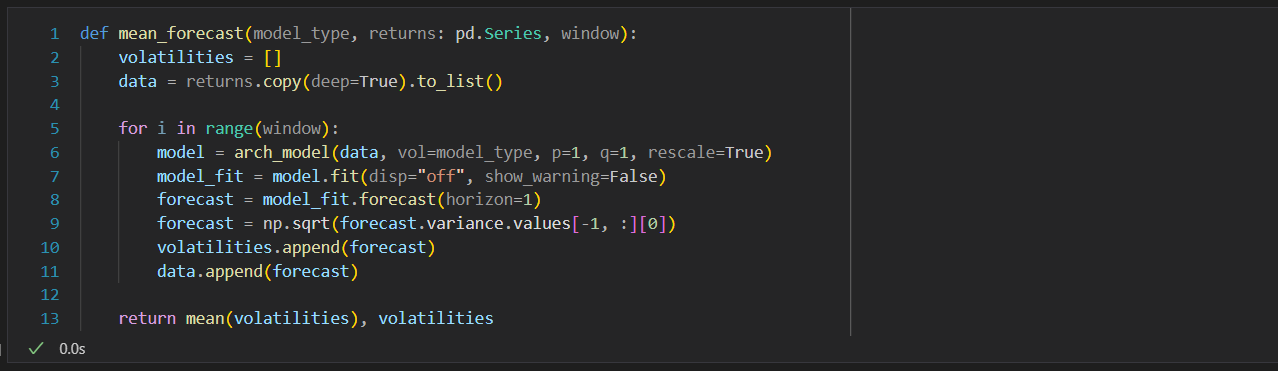
\includegraphics[width=0.4\linewidth]{pic_7}}
	\quad \quad
	\subfloat[
	میانگین نوسانات پیش‌بینی شده
	]{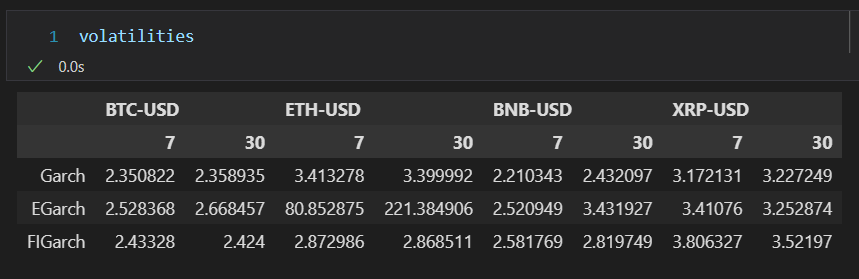
\includegraphics[width=0.4\linewidth]{pic_8}}
	\quad \quad
	\subfloat[
	نمودارهای نوسانات پیش‌بینی شده
	]{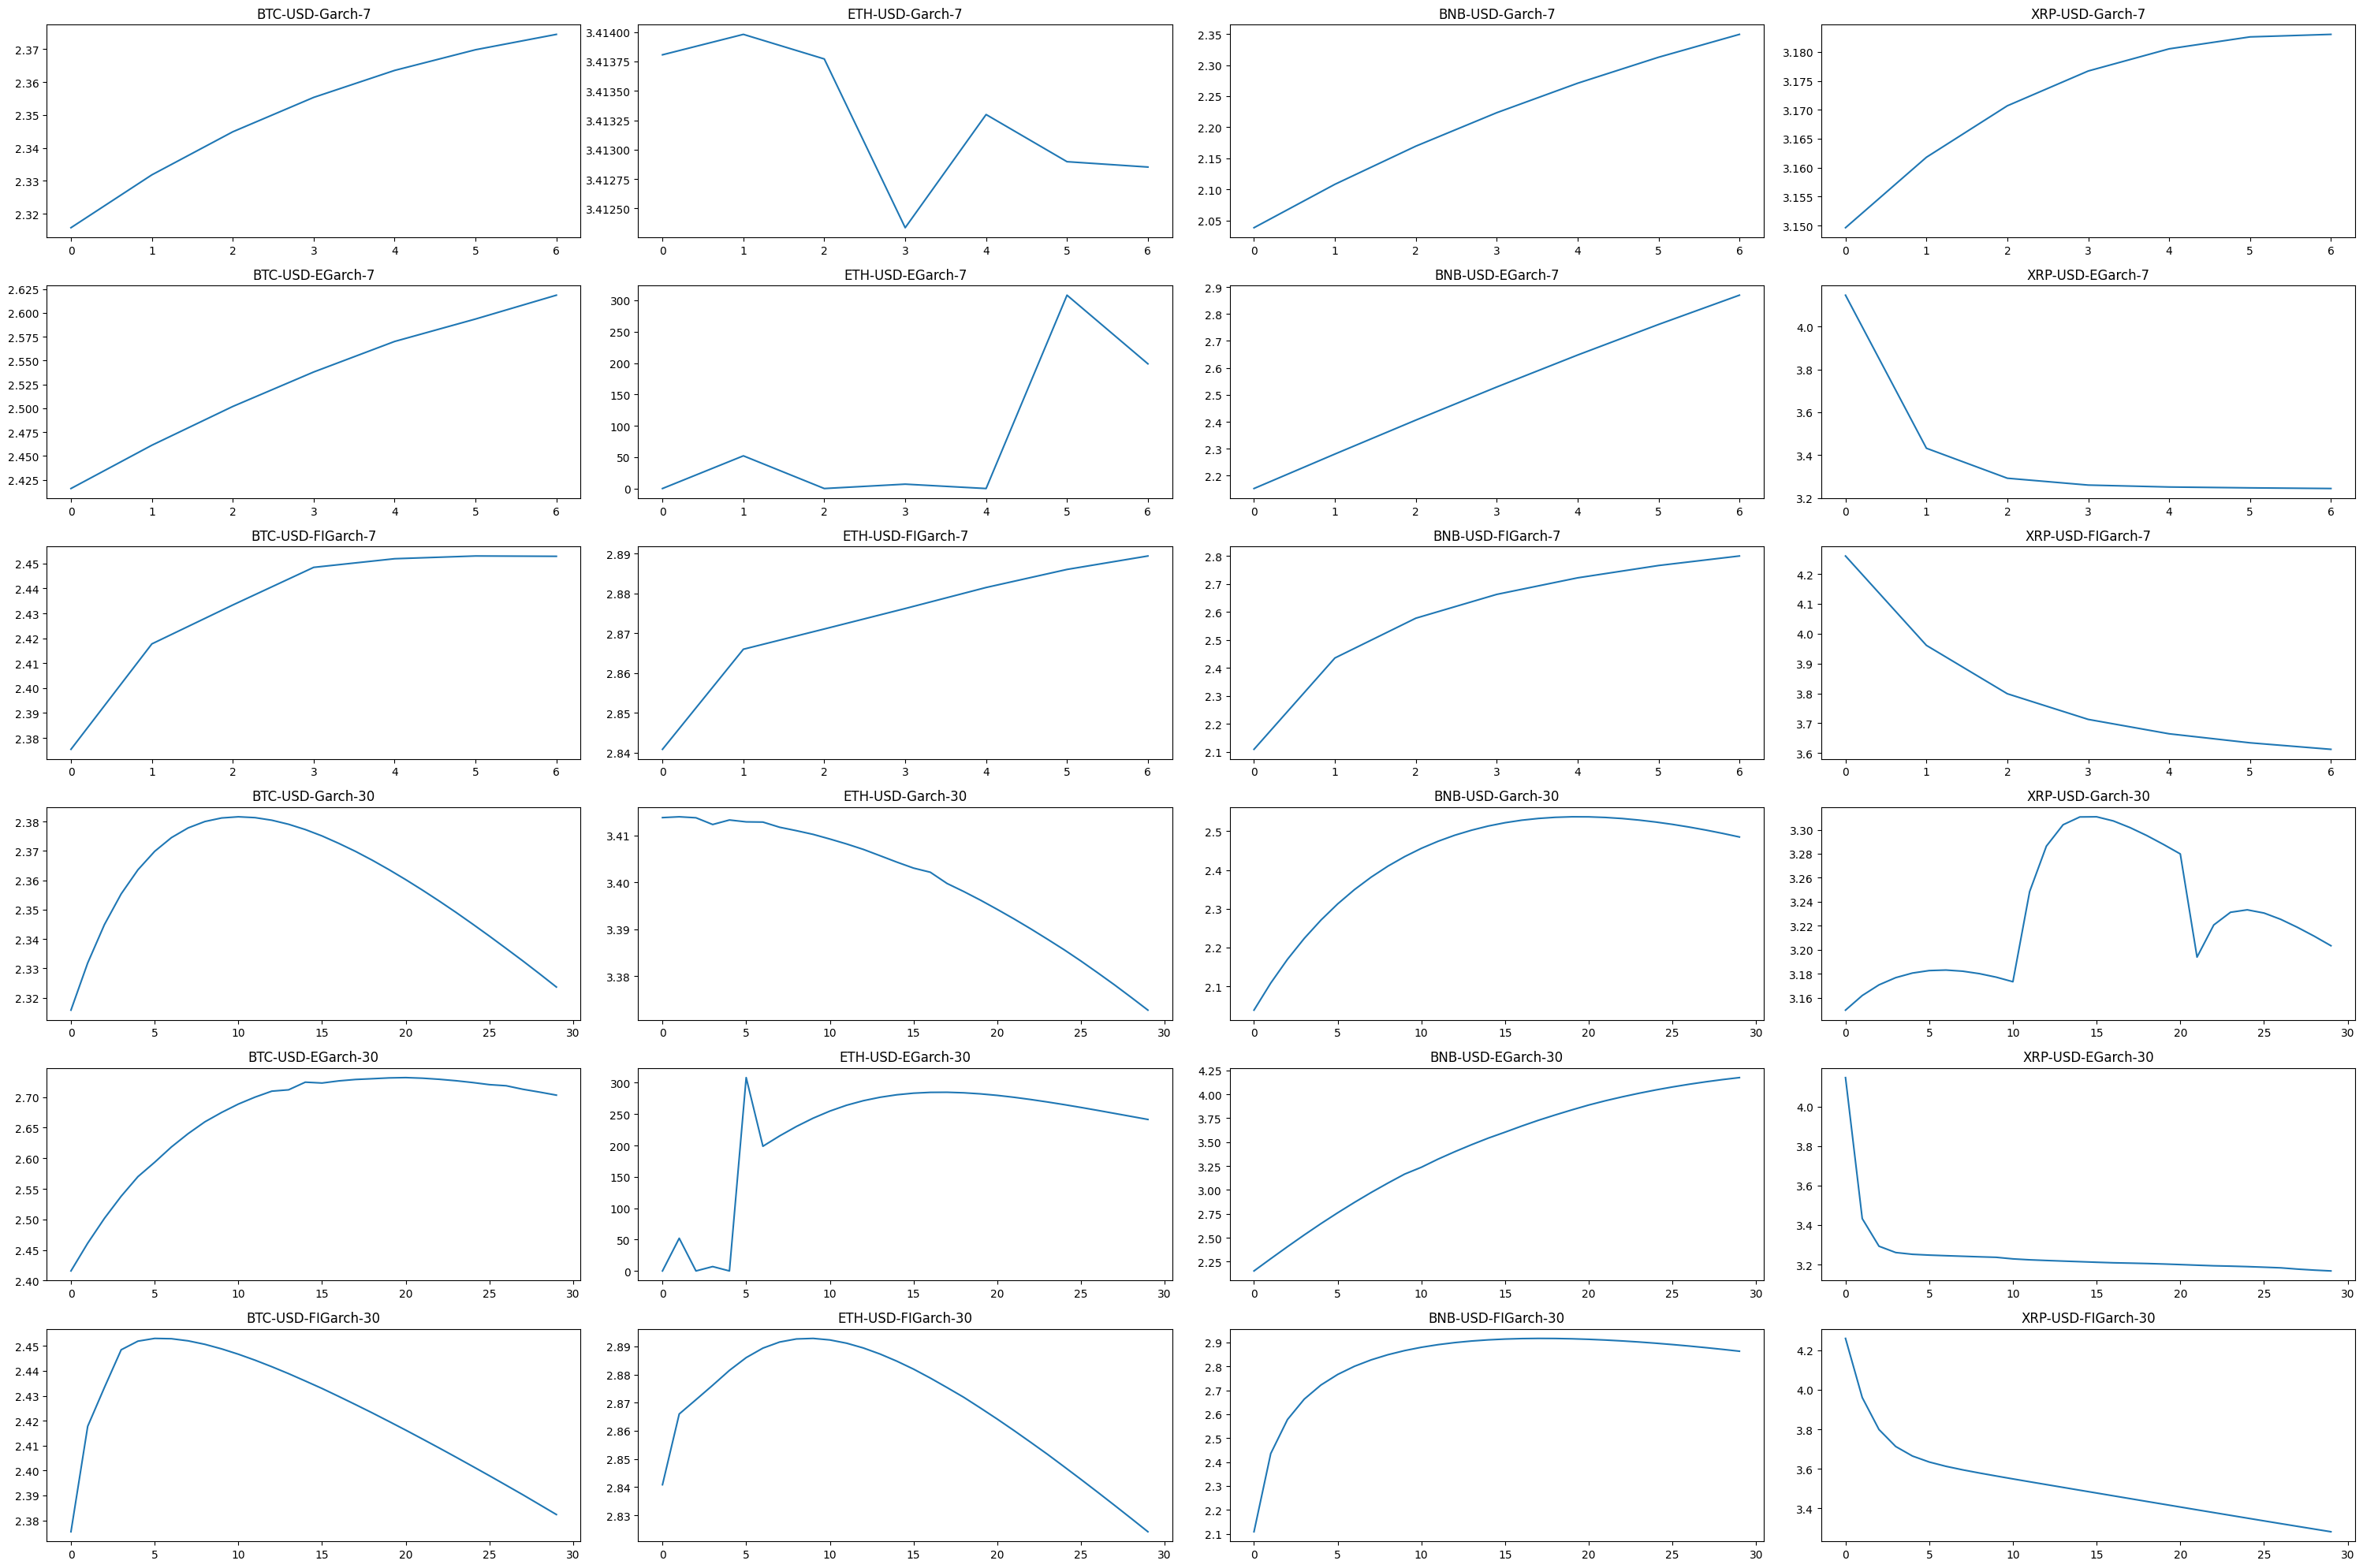
\includegraphics[width=0.4\linewidth]{pic_9}}
\end{figure}
\subsection{پروکسی‌های نوسان}
در ابتدا به پیاده‌سازی هر یک از پروکسی‌ها می‌پردازیم.
\begin{figure}[H]
	\centering
	\subfloat[
	\lr{Historical Volatility}
	]{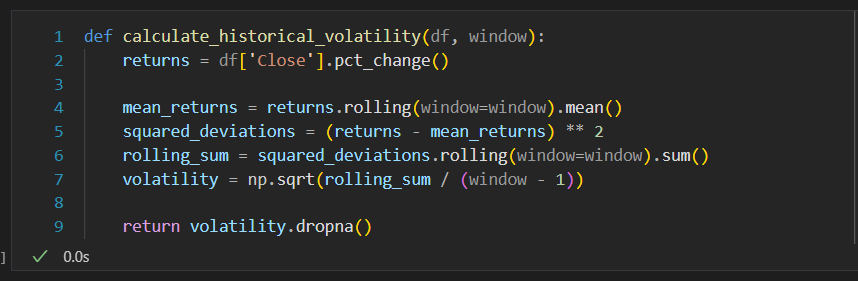
\includegraphics[width=0.4\linewidth]{pic_10}}
	\quad \quad
	\subfloat[
	\lr{Parkinson Volatility}
	]{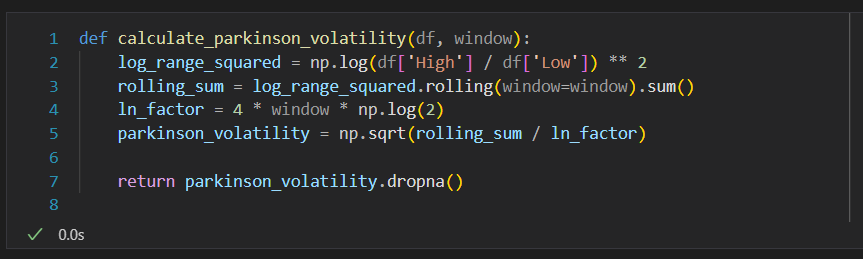
\includegraphics[width=0.4\linewidth]{pic_11}}
	\quad \quad
	\subfloat[
	\lr{Garman-Klass Volatility}
	]{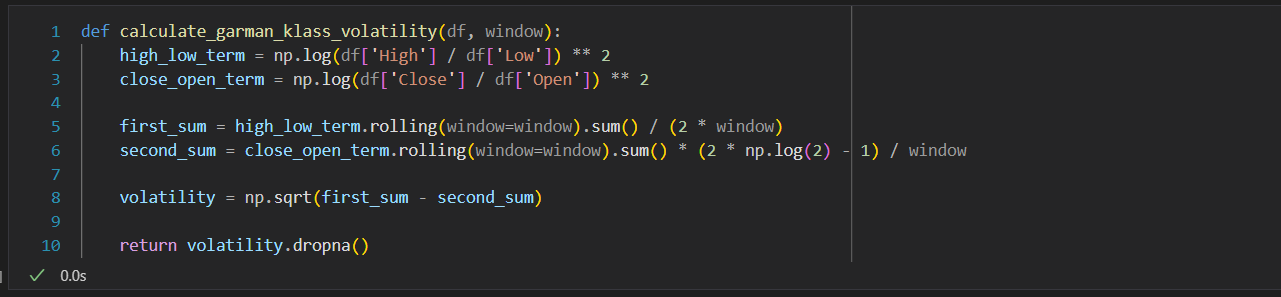
\includegraphics[width=0.4\linewidth]{pic_12}}
	\quad \quad
	\subfloat[
	\lr{Yang-Zhang Volatility}
	]{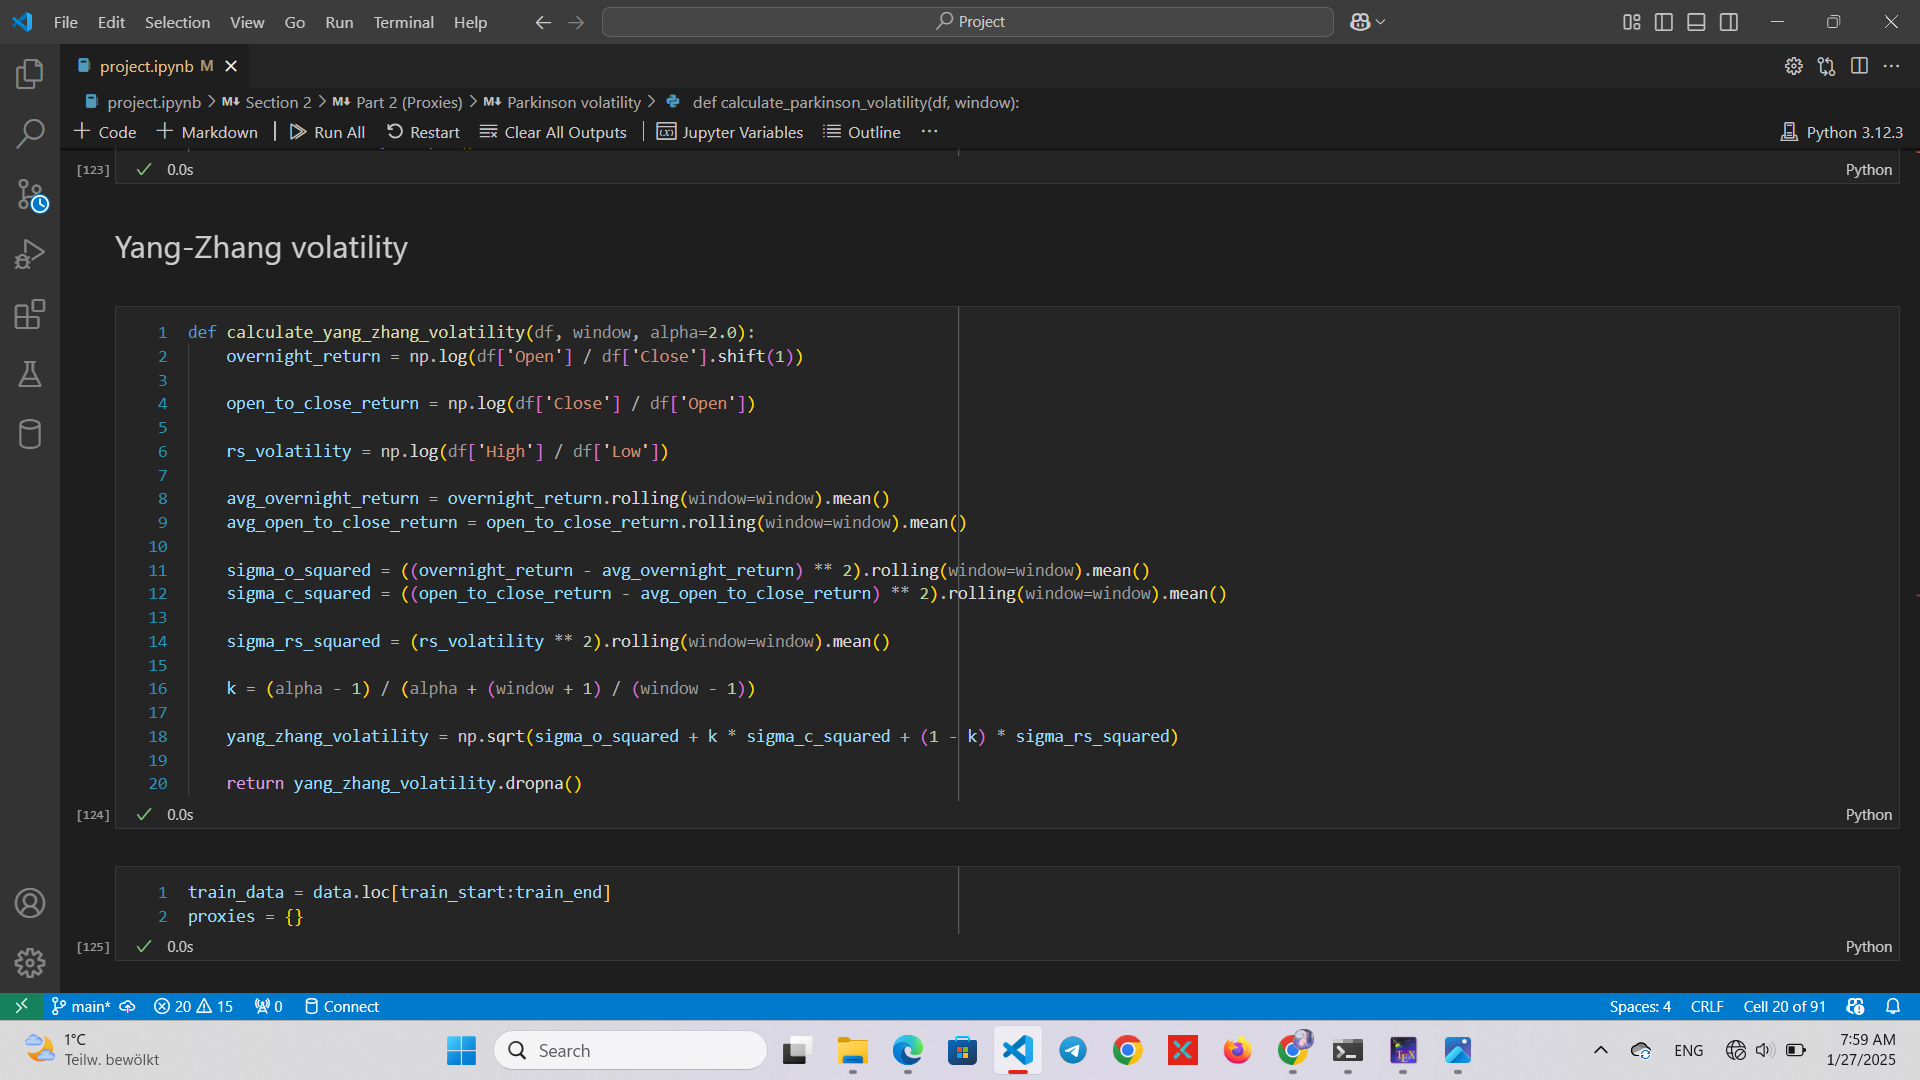
\includegraphics[width=0.4\linewidth]{pic_13}}
\end{figure}
سپس به محاسبه تخمین نوسانات دو دو پنجره زمانی ۷ و ۳۰ روزه می‌پردازیم.
\begin{figure}[H]
	\centering
	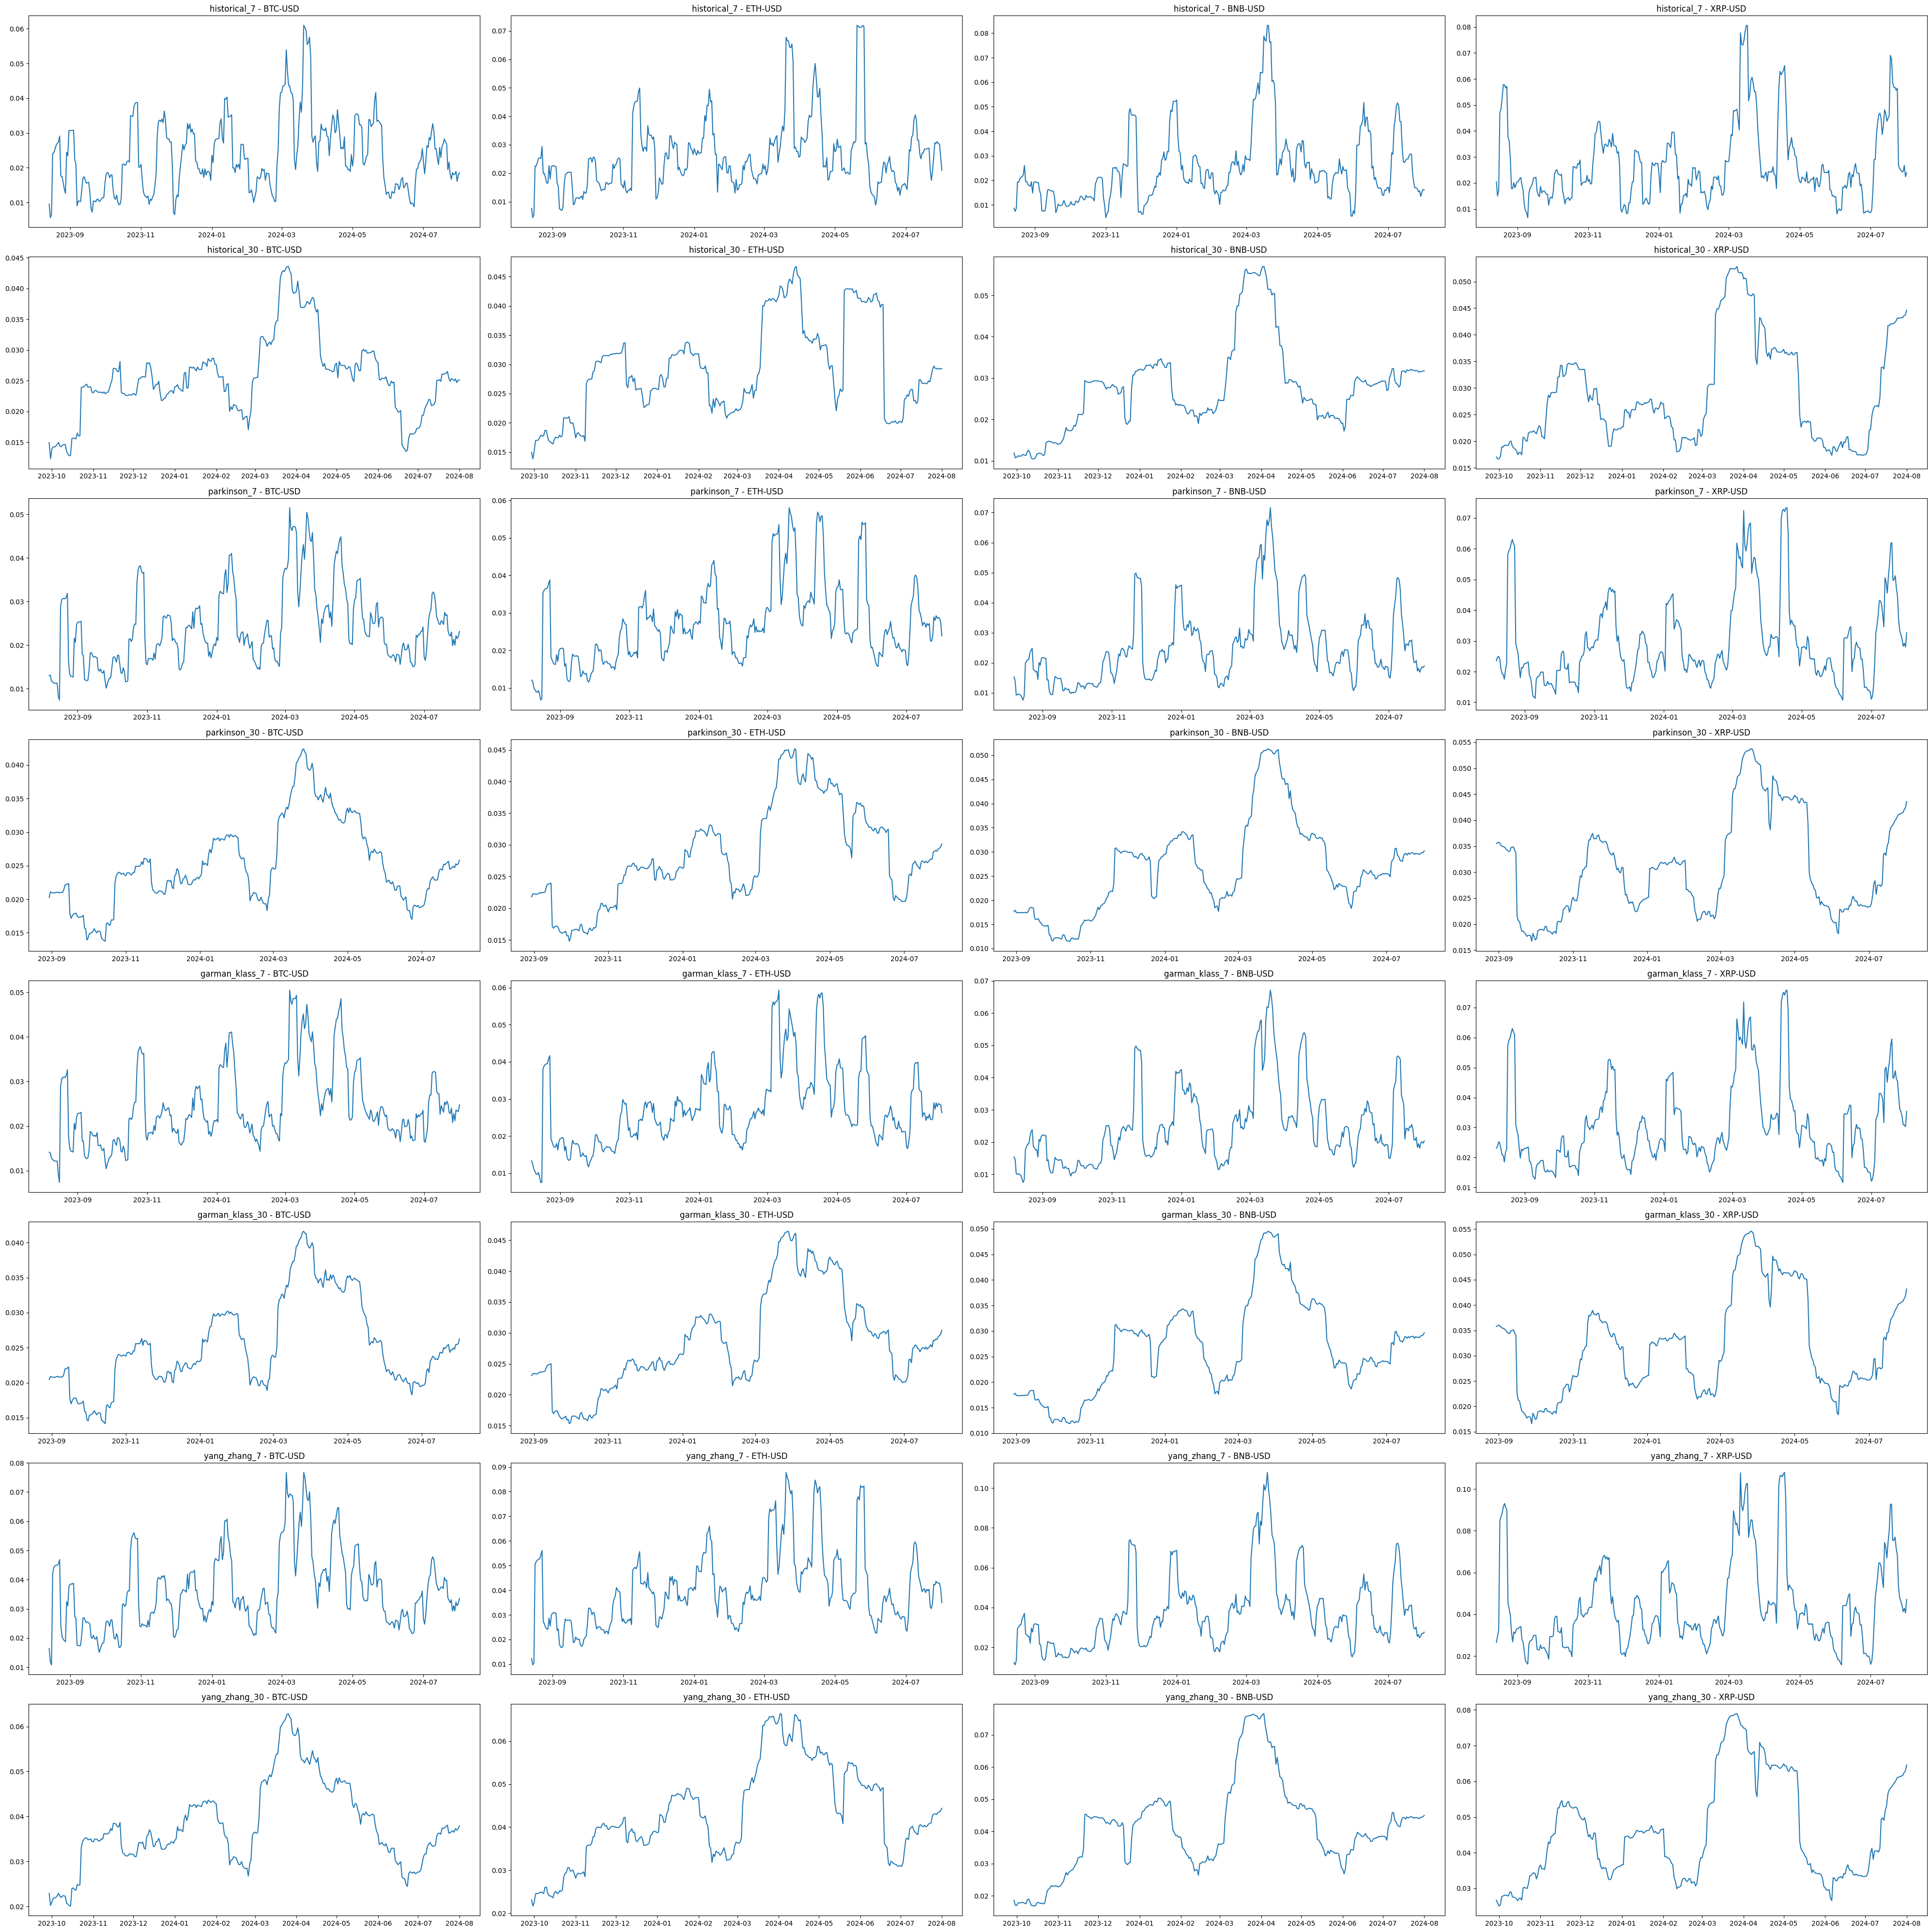
\includegraphics[width=0.9\linewidth]{pic_14}
	\caption{نوسانات تخمین زده شده برای رمزارزهای مختلف}
\end{figure}
\section{روش وزن‌دهی و بهینه‌سازی پورتفولیو (\lr{Portfolio Optimization})}
\subsection{ادغام سری‌های نوسان}
در این بخش قصد داریم تا میانگین سری‌ها را محاسبه کنیم.
\begin{figure}[H]
	\centering
	\subfloat[
	\lr{Statistical Models}
	]{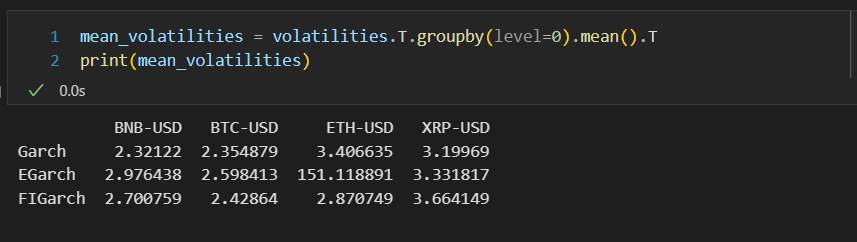
\includegraphics[width=0.4\linewidth]{pic_15}}
	\quad \quad
	\subfloat[
	\lr{Proxies}
	]{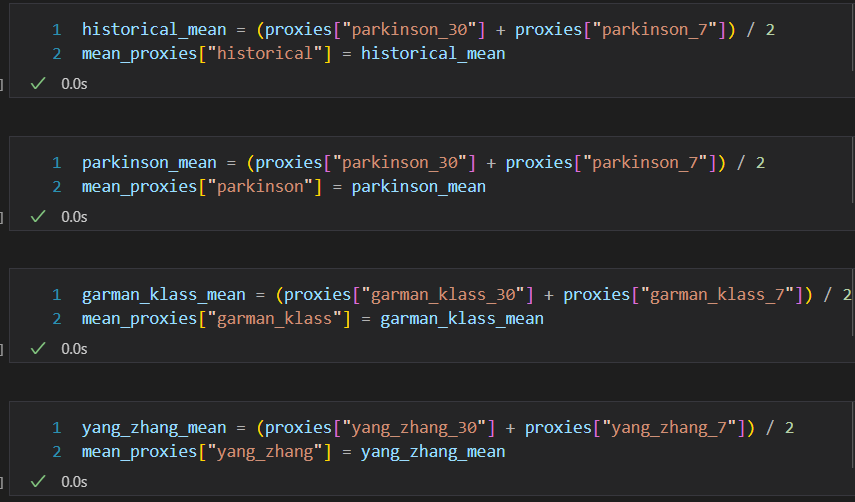
\includegraphics[width=0.4\linewidth]{pic_16}}
	\subfloat[
	نمودارهای میانگین‌های سری نوسانات برای \lr{Proxies}
	]{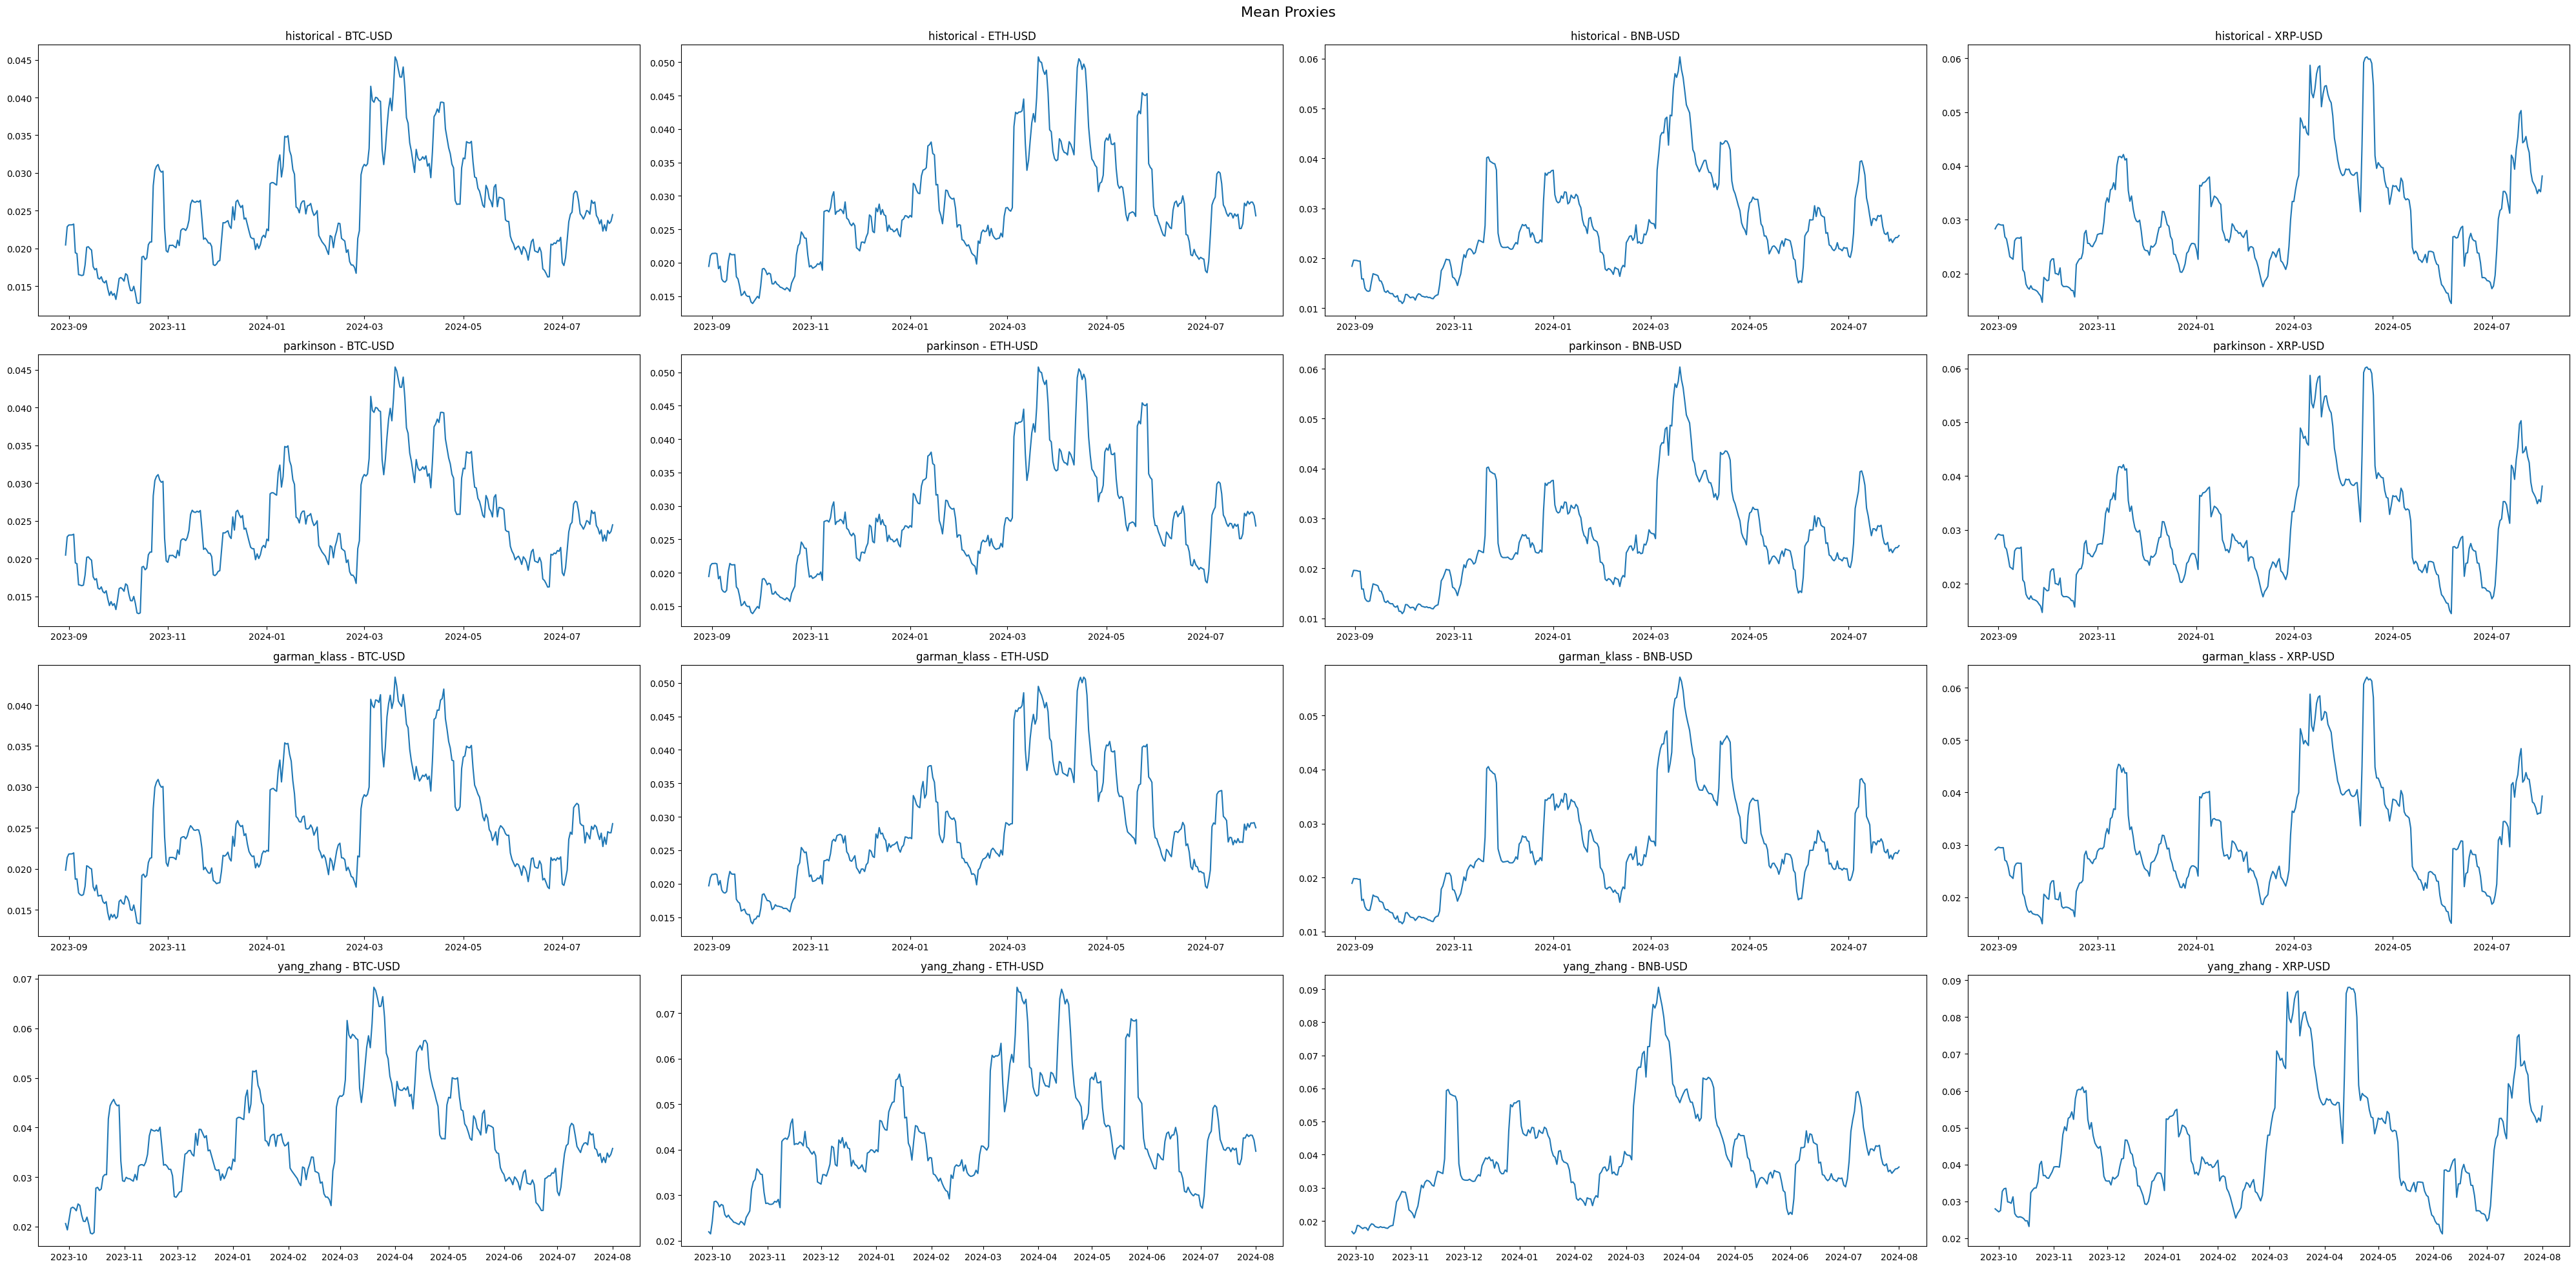
\includegraphics[width=0.4\linewidth]{pic_17}}
\end{figure}
\subsection{بهینه‌سازی پورتفولیو برای هر دسته}
حال به بهینه‌سازی پورتفولیو با توجه به نوسانات می‌پردازیم.
\subsubsection{\lr{Statistical Models}}
در ابتدا \lr{Market Cap} را بدست می‌آوریم.
\begin{figure}[H]
	\centering
	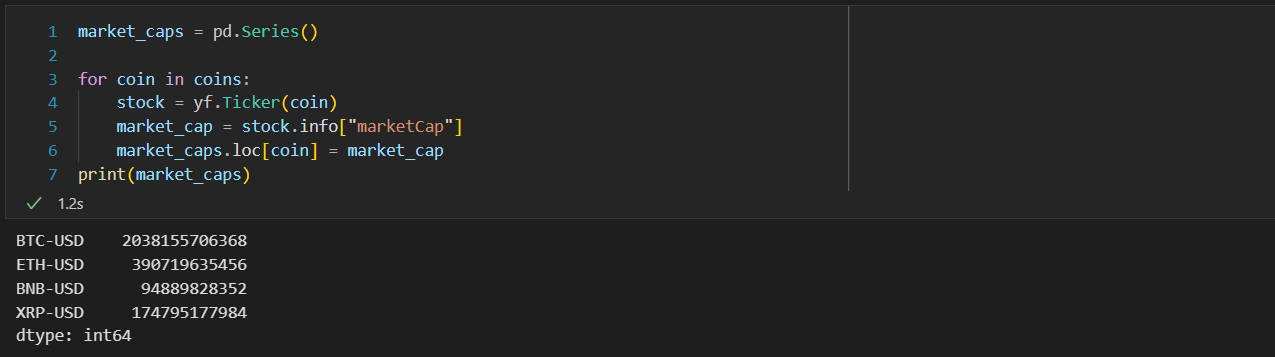
\includegraphics[width=0.9\linewidth]{pic_18}
\end{figure}
سپس به محاسبه کواریانس مقادیر و \lr{risk-aversion} می‌پردازیم تا وزن‌های اولیه‌ی پورتفولیو بدست آیند. این وزن‌ها سپس توسط مدل تغییر خواهند کرد.
\begin{figure}[H]
	\centering
	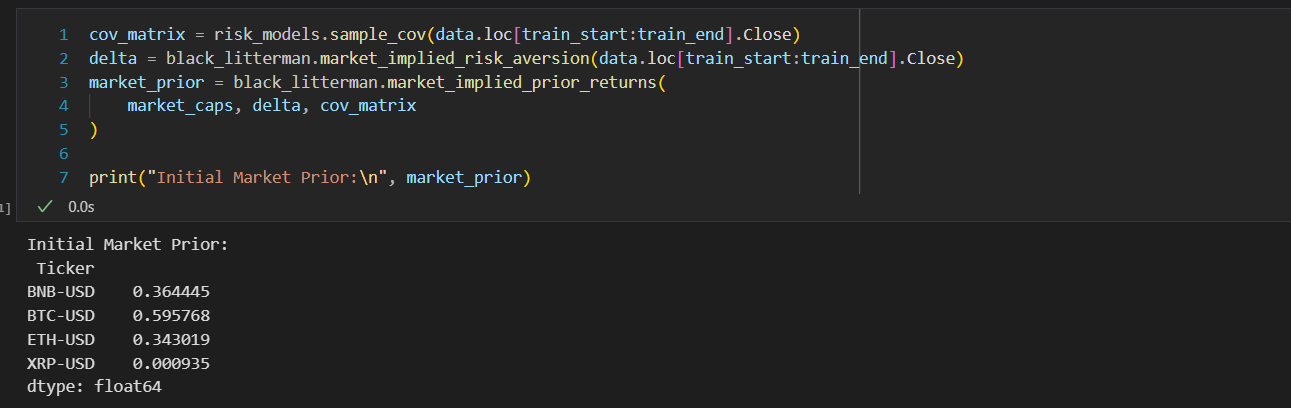
\includegraphics[width=0.9\linewidth]{pic_19}
\end{figure}
حال به محاسبه وزن‌های بهینه‌شده توسط مدل می‌پردازیم. این وزن‌ها براساس نمودار \lr{Efficient Frontier} و برای متریک \lr{Max Sharpe Ratio} بدست آمده اند.
\begin{figure}[H]
	\centering
	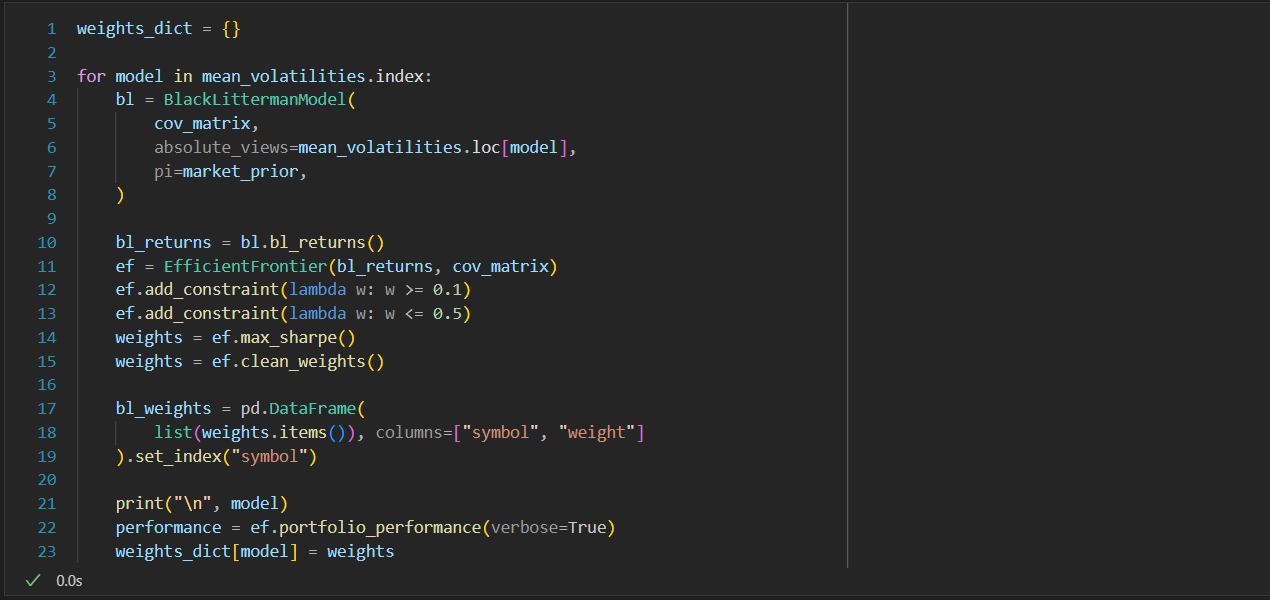
\includegraphics[width=0.9\linewidth]{pic_20}
\end{figure}
\begin{figure}[H]
	\centering
	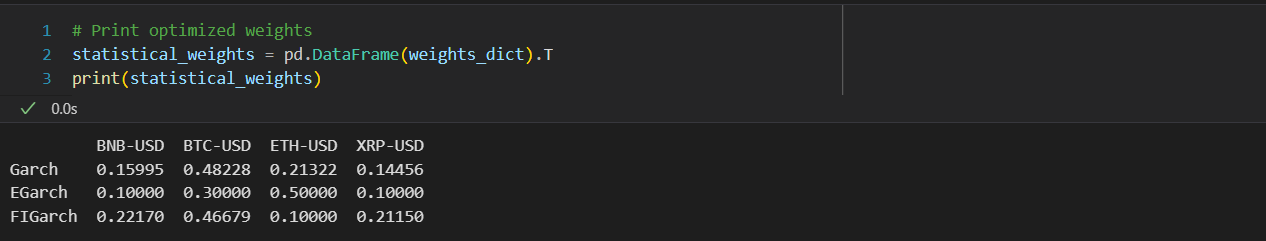
\includegraphics[width=0.9\linewidth]{pic_21}
	\caption{وزن‌های نهایی بدست آمده برای مدل‌های آماری}
\end{figure}
\subsubsection{\lr{Proxies}}
برای پروکسی‌ها هم مشابه مدل‌های آماری، به محاسبه \lr{Market Cap}، \lr{Covariance Matrix} و \lr{ًRisk-Aversion} می‌پردازیم تا وزن‌های اولیه بدست آیند. سپس به محاسبه وزن‌های بهینه می‌پردازیم.
\begin{figure}[H]
	\centering
	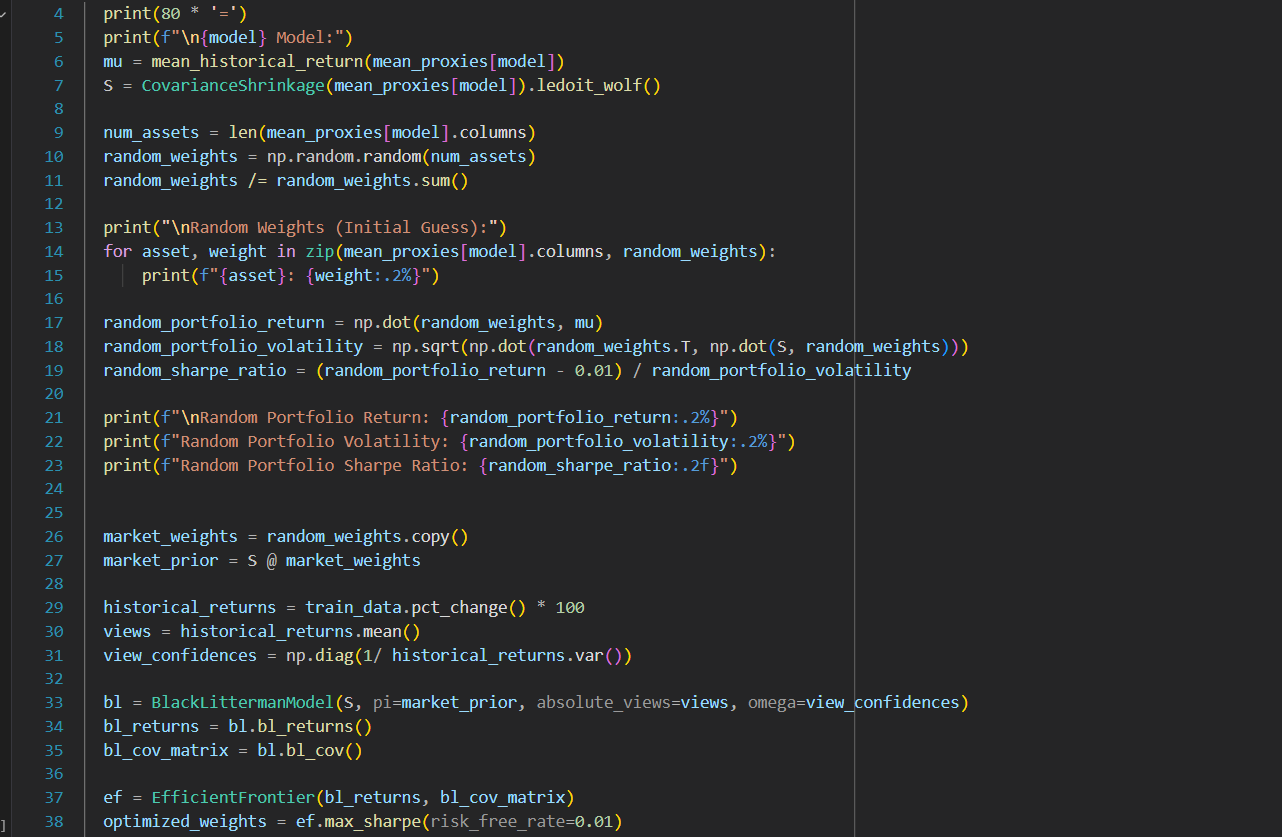
\includegraphics[width=0.9\linewidth]{pic_23}
\end{figure}
\begin{figure}[H]
	\centering
	\subfloat[
	نمونه‌ای از یک خروجی برای \lr{Historical Proxy}
	]{
	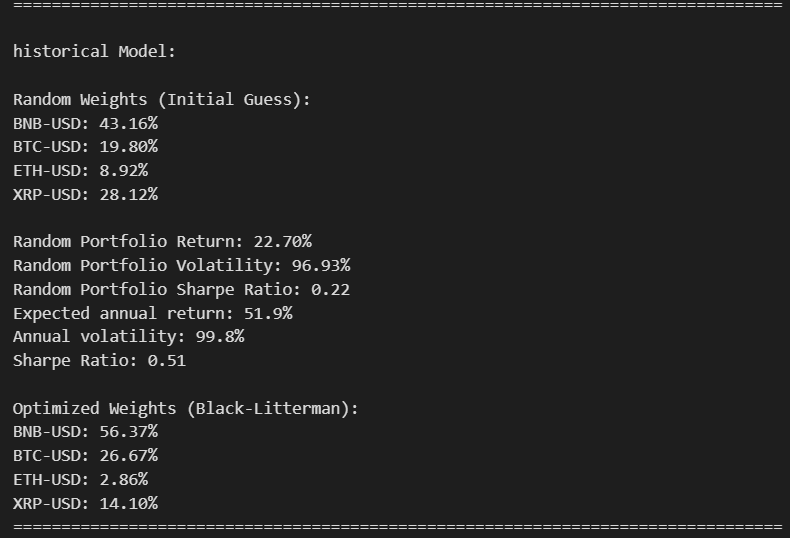
\includegraphics[width=0.4\linewidth]{pic_24}}
	\quad \quad
	\subfloat[
	وزن‌های محاسبه شده
	]{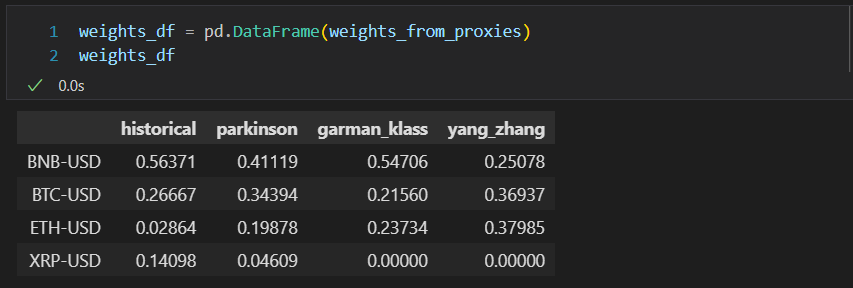
\includegraphics[width=0.4\linewidth]{pic_25}}
\end{figure}
\section{استراتژی و استفاده از پورتفولیو}
در این بخش، در ابتدا به پیاده‌سازی استراتژی و متریک‌های ذکرشده می‌پردازیم.
\begin{figure}[H]
	\centering
	\subfloat[
	استراتژی \lr{Buy and Hold}
	]{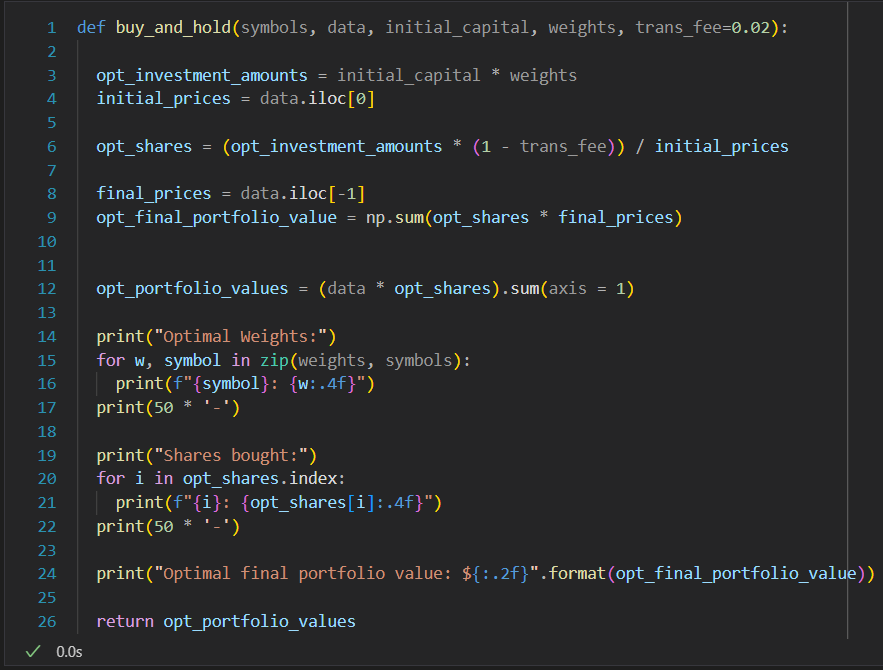
\includegraphics[width=0.4\linewidth]{pic_26}}
	\quad \quad
	\subfloat[
	متریک‌های \lr{Sharpe Ratio}, \lr{Net Profit} و \lr{Max Drawdown}
	]{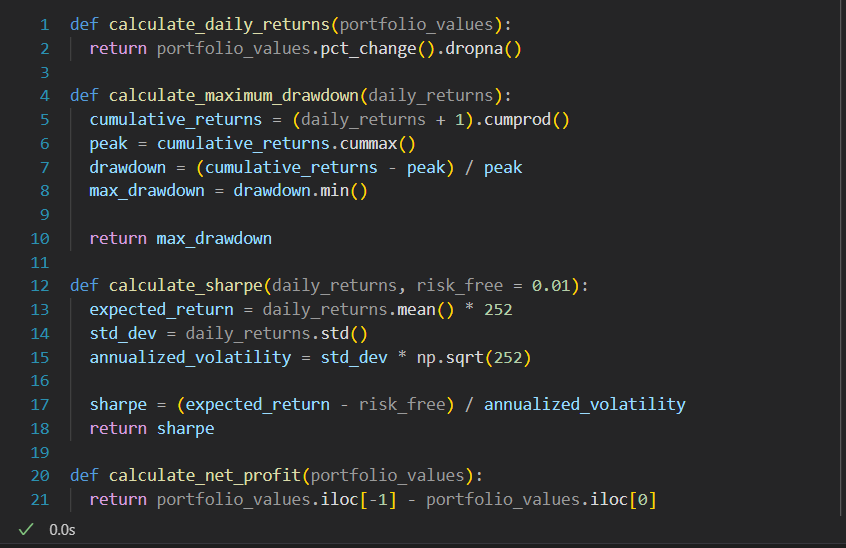
\includegraphics[width=0.4\linewidth]{pic_27}}
\end{figure}
سپس به اجرای استراتژی روی وزن‌های بدست آمده از روش‌های مختلف می‌پردازیم. نمودارهای قیمتی در ادامه خواهند آمد و مفادیر وزن‌ها نیز از نوت‌بوک قابل دسترسی اند.
\begin{figure}[H]
	\centering
	\subfloat[
	اجرای استراتژی برای وزن‌های مدل‌های آماری روی داده آموزش
	]{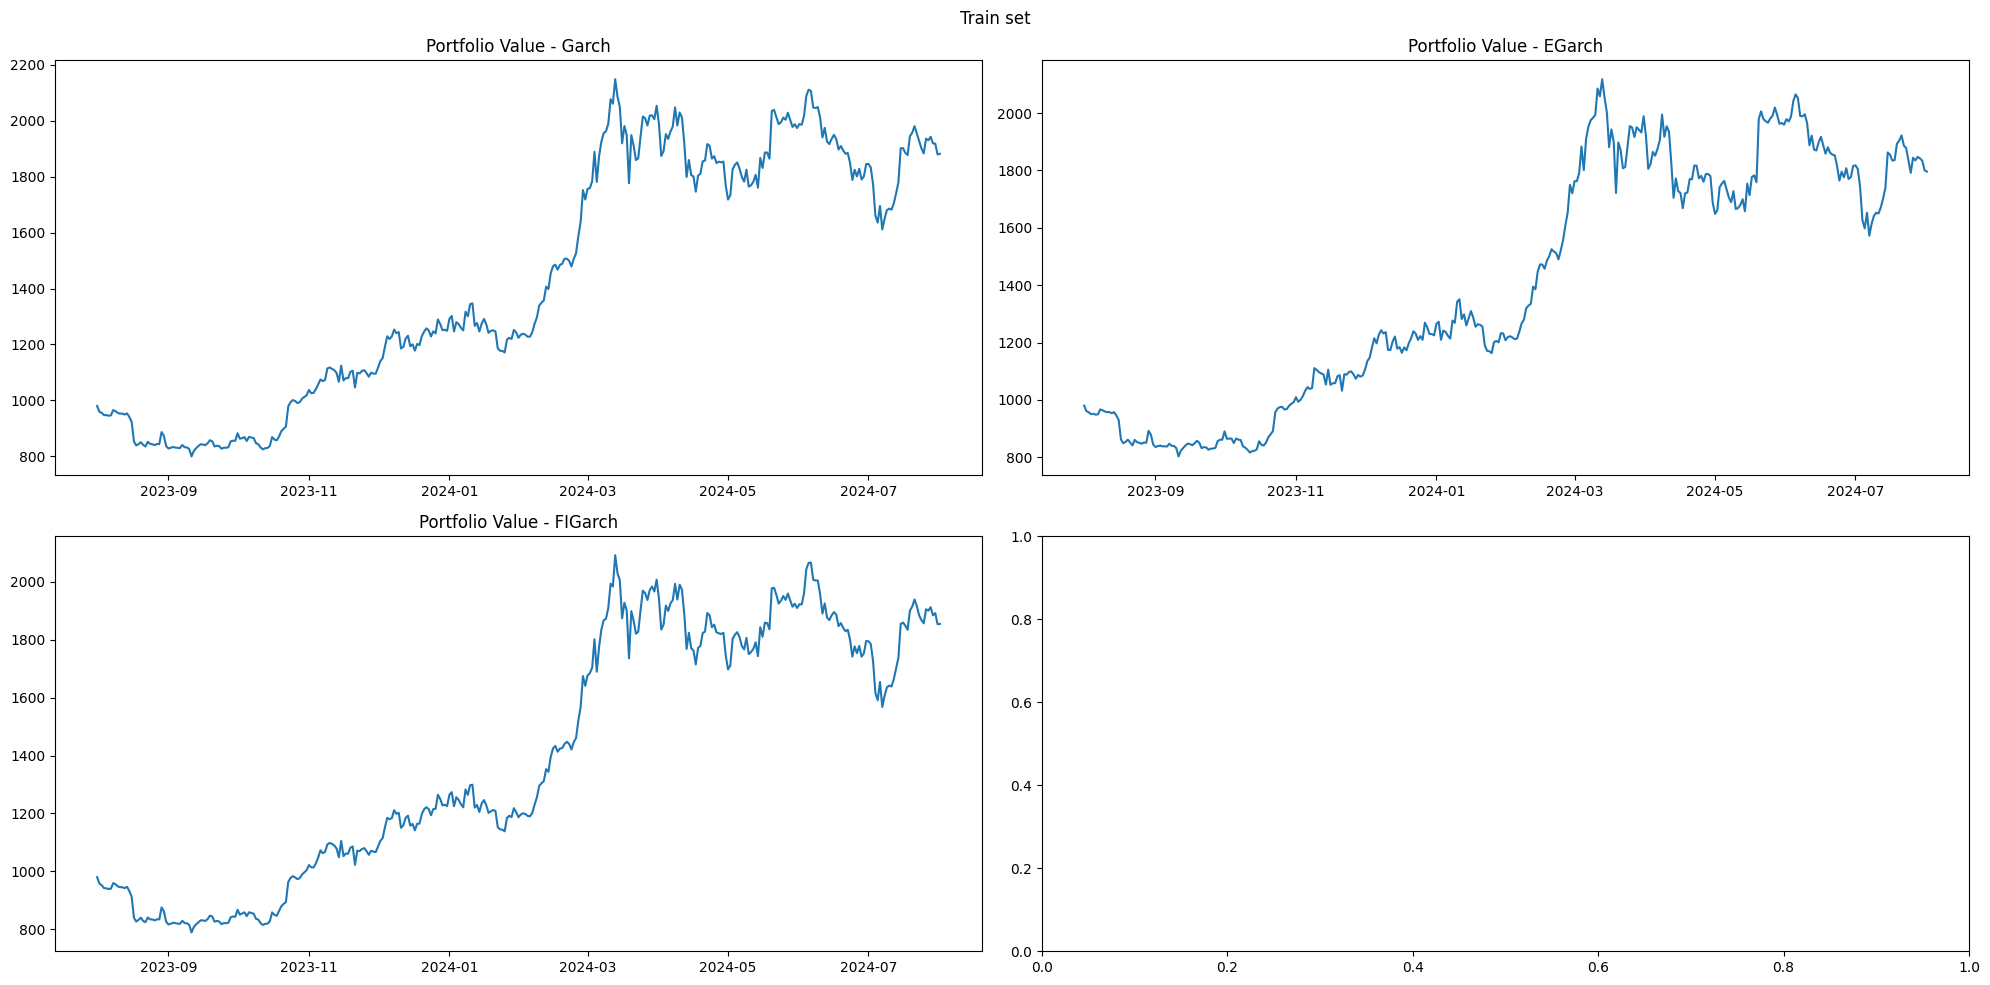
\includegraphics[width=0.4\linewidth]{pic_28}}
	\quad \quad
	\subfloat[
	اجرای استراتژی برای وزن‌های پروکسی‌ها روی داده آموزش
	]{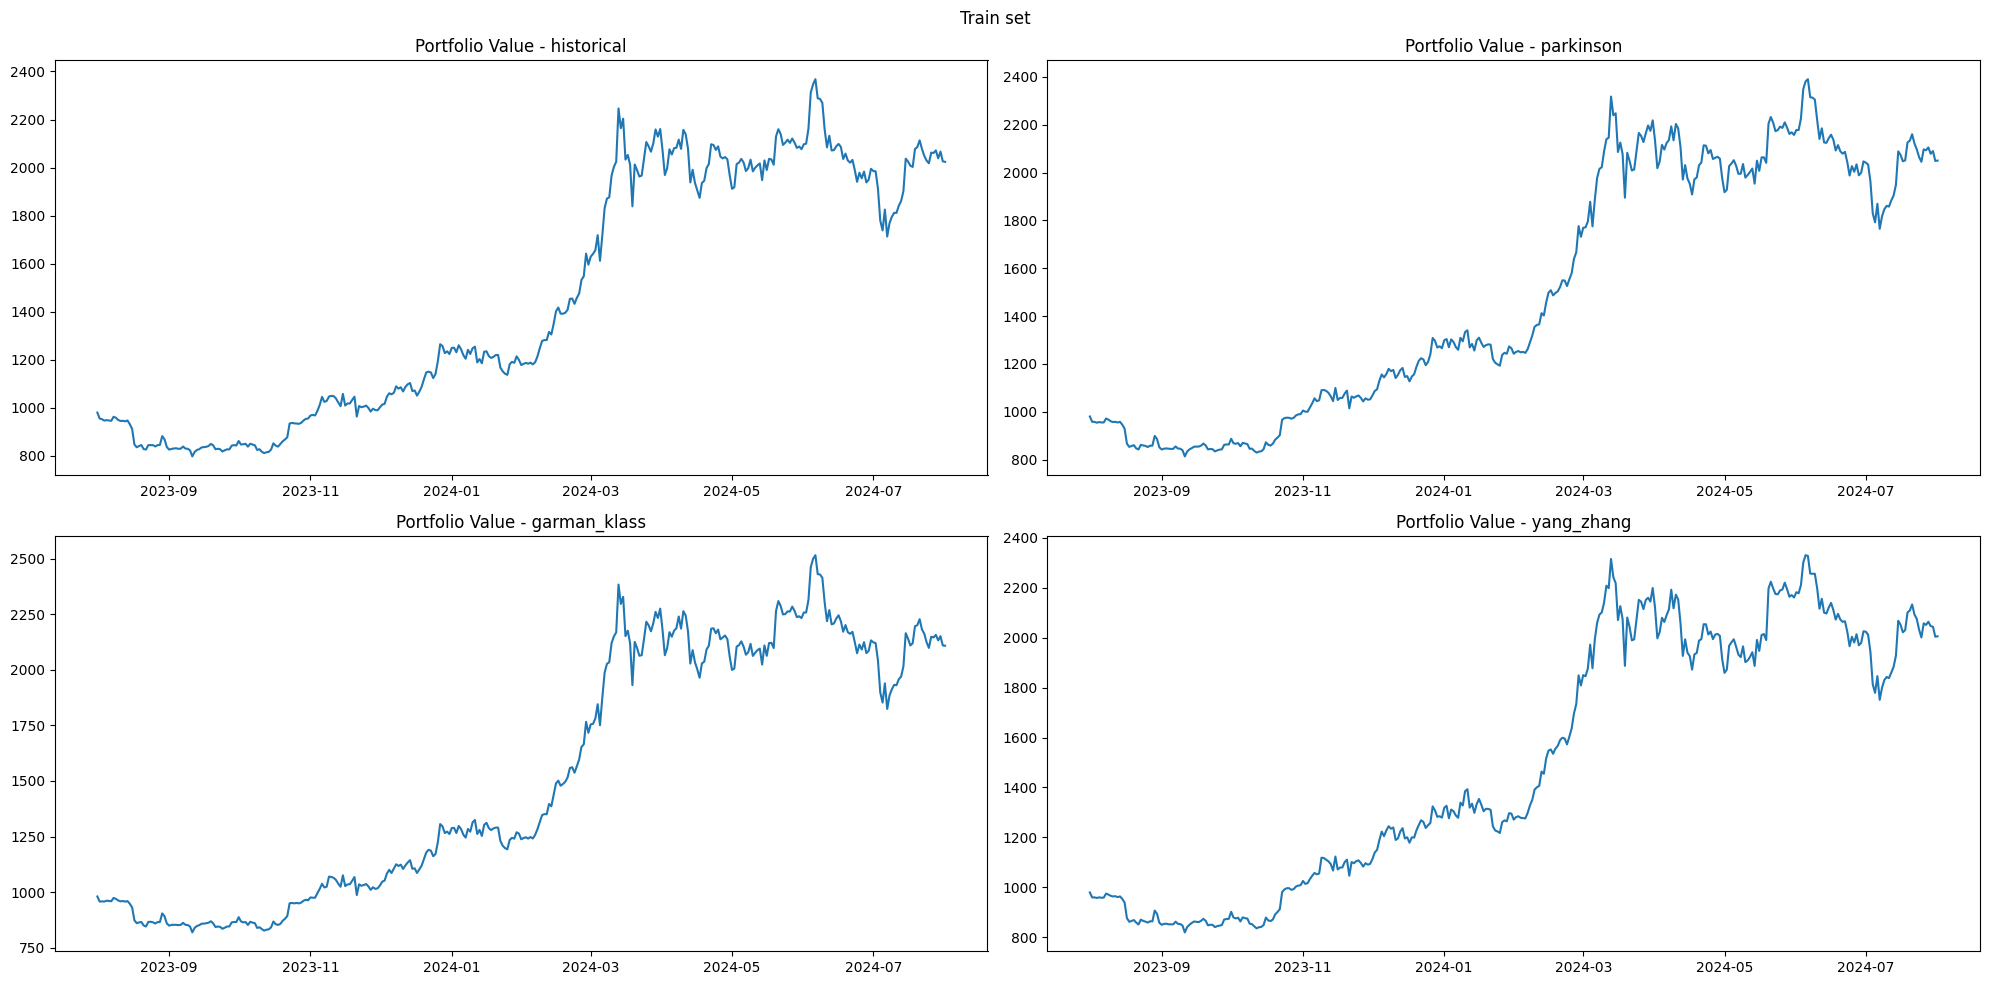
\includegraphics[width=0.4\linewidth]{pic_29}}
	\quad \quad
	\subfloat[
	اجرای استراتژی برای وزن‌های مدل‌های آماری روی داده تست
	]{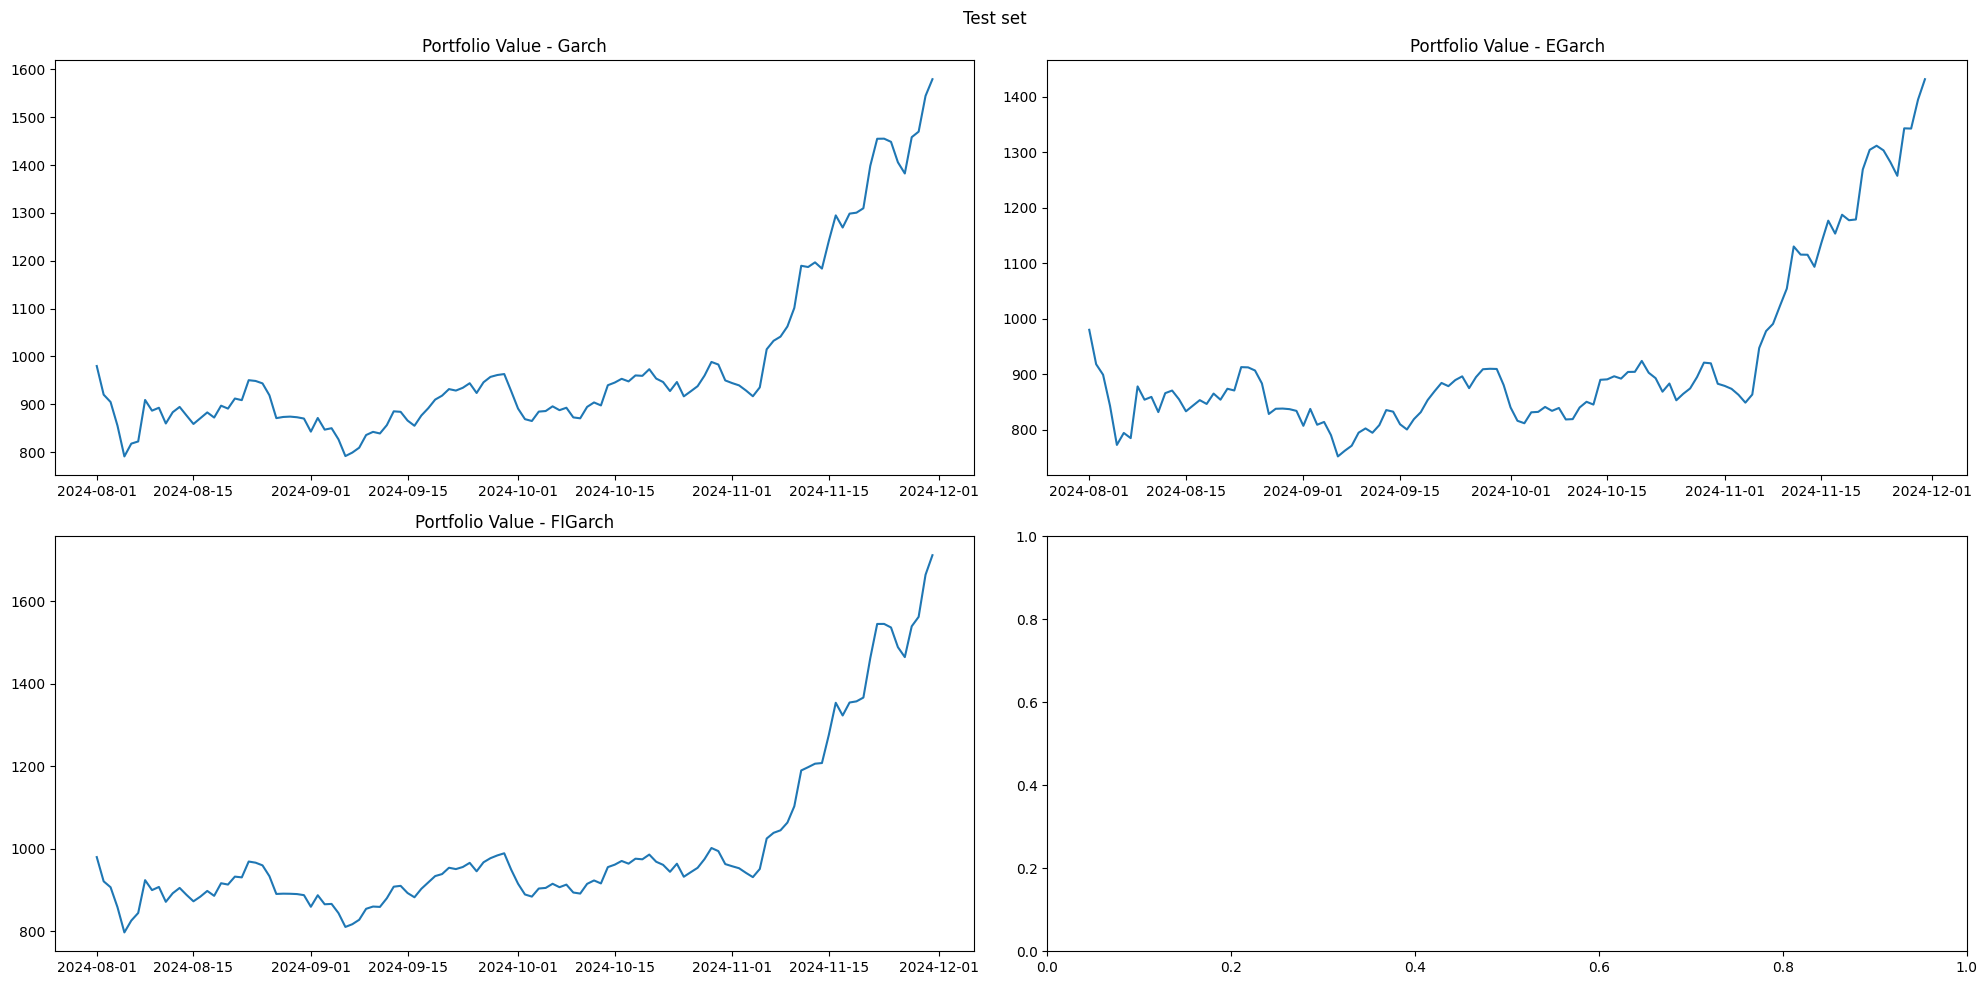
\includegraphics[width=0.4\linewidth]{pic_30}}
	\quad \quad
	\subfloat[
	اجرای استراتژی برای وزن‌های پروکسی‌ها روی داده تست
	]{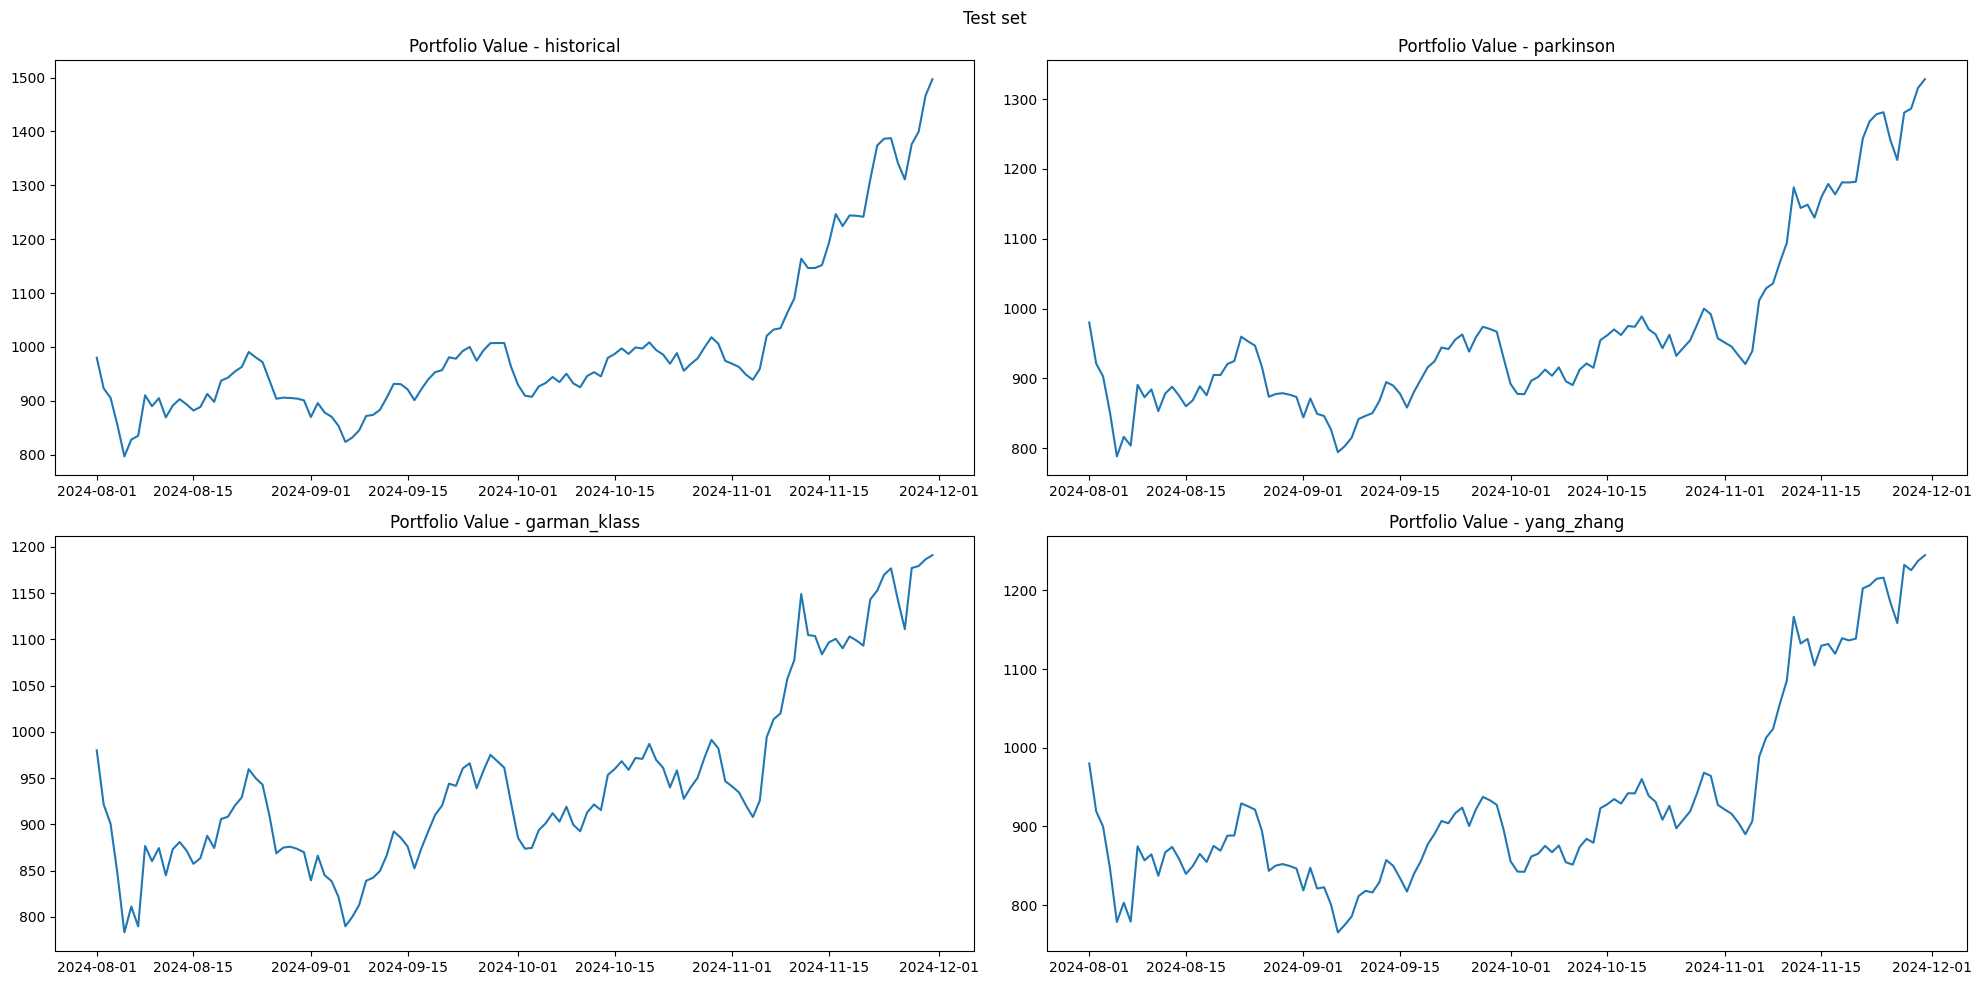
\includegraphics[width=0.4\linewidth]{pic_31}}
\end{figure}
\section{تحلیل نتایج}
با توجه به معیارهای گزارش شده (در نوت‌بوک) برای هر دسته وزن و تخمین‌گر نوسان، سری نوسانی \lr{FIGarch} عملکرد بهتری نسبت به بقیه دارد زیرا هم نسبت \lr{Sharpe Ratio} بهتری نسبت به بقیه دارد و هم اینکه مقدار \lr{Net Profit} آن بیشتر است.

حال به رسم نمودارهای ذکر شده برای دسته با خروجی بهینه می‌پردازیم.
\begin{figure}[H]
	\centering
	\subfloat[
	نمودار \lr{Equity}
	]{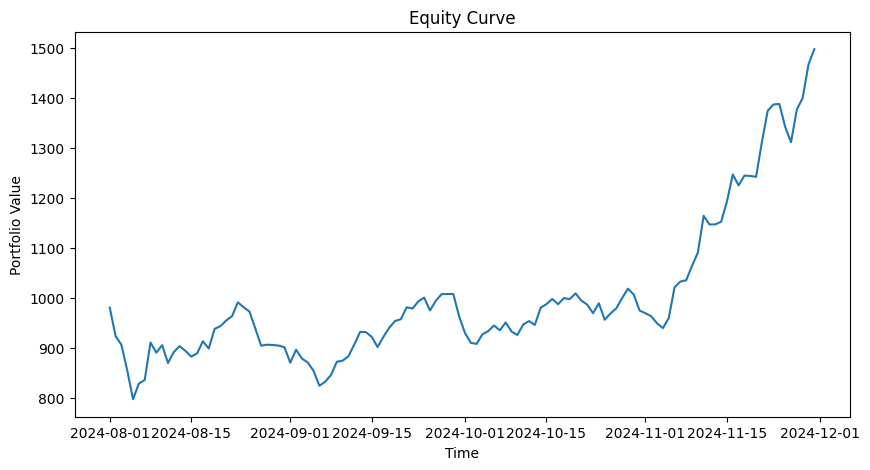
\includegraphics[width=0.4\linewidth]{pic_32}}
	\quad \quad
	\subfloat[
	نمودار \lr{Portfolio Allocation}
	]{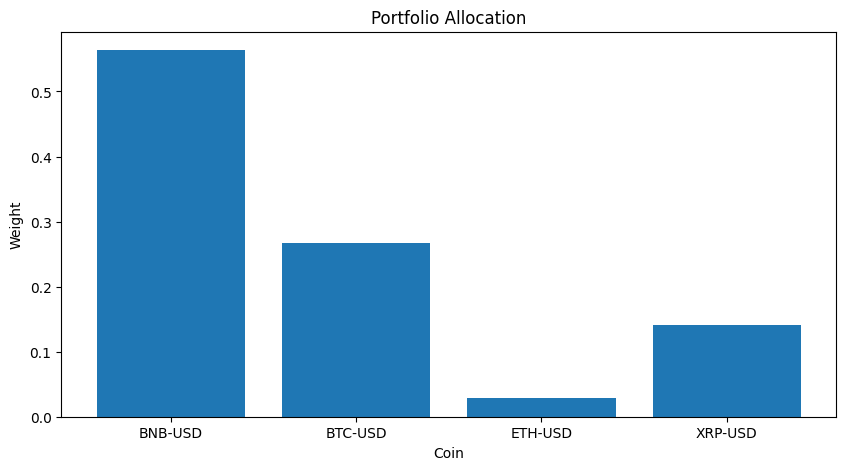
\includegraphics[width=0.4\linewidth]{pic_33}}
	\quad \quad
	\subfloat[
	نمودار \lr{Volatility Dynamics over time}
	]{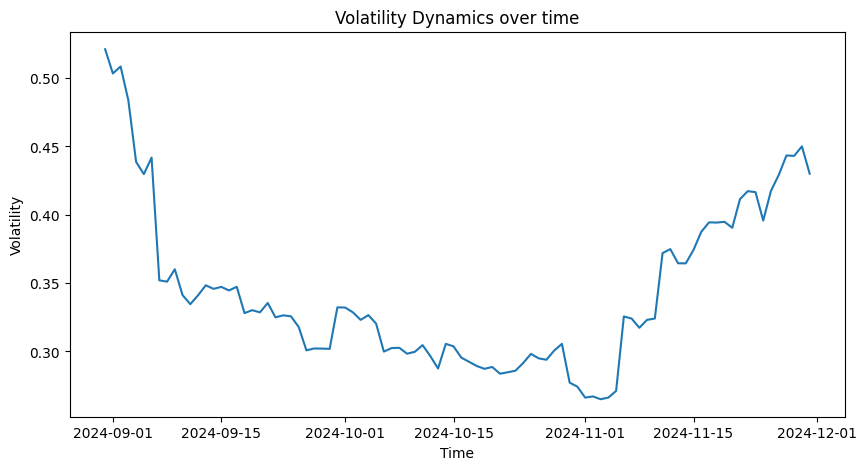
\includegraphics[width=0.4\linewidth]{pic_34}}
	\quad \quad
	\subfloat[
	نمودار \lr{Confidence Intervals of Portfolio Estimates}
	]{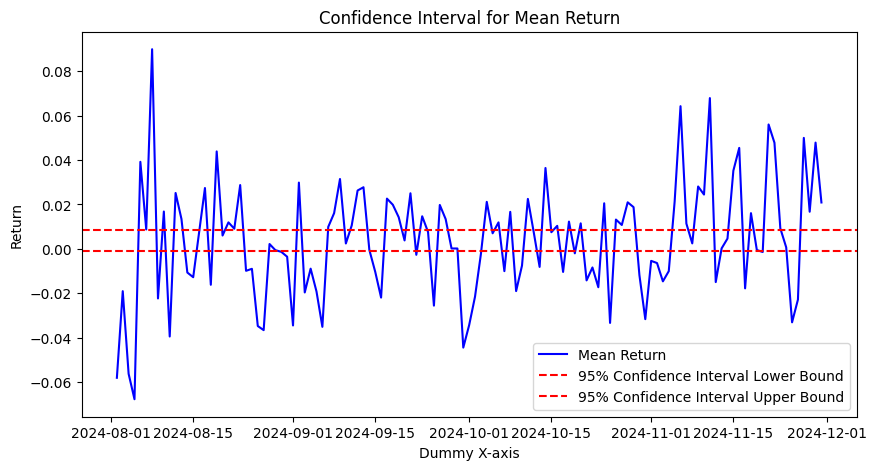
\includegraphics[width=0.4\linewidth]{pic_35}}
	\quad \quad
	\subfloat[
	نمودار \lr{Cumulative Return}
	]{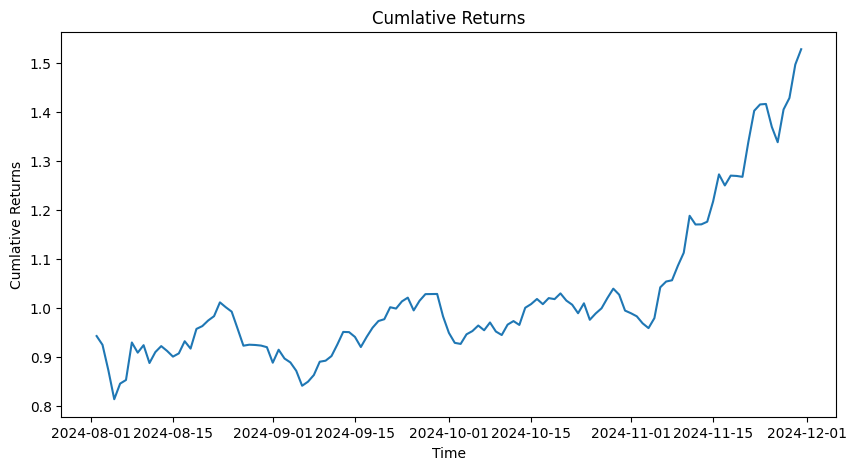
\includegraphics[width=0.4\linewidth]{pic_36}}
\end{figure}
\end{document}